% !TeX program = xelatex
\documentclass[11pt,a4paper]{article}

\usepackage[a4paper,top=25.4mm,bottom=25.4mm,left=25.4mm,right=25.4mm,headheight=14pt]{geometry}
% Overleaf imports default to pdfLaTeX, while the preferred build uses
% XeLaTeX. Keep the document compilable with either engine.
\usepackage{iftex}
\ifPDFTeX
  \usepackage[T1]{fontenc}
  \usepackage[utf8]{inputenc}
  \usepackage{newpxtext,newpxmath}
\else
  \usepackage{fontspec}
  \usepackage{unicode-math}
  \setmainfont{texgyrepagella-regular.otf}[
    BoldFont=texgyrepagella-bold.otf,
    ItalicFont=texgyrepagella-italic.otf,
    BoldItalicFont=texgyrepagella-bolditalic.otf
  ]
  \setmathfont{texgyrepagella-math.otf}
\fi
\usepackage{microtype}
\usepackage{setspace}
\setstretch{1.5}
\setlength{\parindent}{0pt}
\setlength{\parskip}{0.45em plus 0.1em minus 0.1em}

\usepackage{amsmath}
\usepackage{graphicx}
\usepackage{xcolor}
\usepackage{longtable,booktabs,array,tabularx,makecell}
\usepackage{calc}
\usepackage{ragged2e}
\usepackage{caption}
\usepackage{etoolbox}
\usepackage{footnotehyper}
\usepackage{needspace}
\usepackage{titlesec}
\usepackage{fancyhdr}
\usepackage{xurl}
\usepackage[hidelinks]{hyperref}
\usepackage{bookmark}

\renewcommand{\theHequation}{\arabic{equation}}

\hypersetup{
  pdftitle={Restrictiveness and Skill Composition},
  pdfauthor={Toprak Yetimoglu},
  pdfsubject={MSc Thesis in Economics, International Finance and Trade},
  colorlinks=false
}

% The source already carries section numbers in its headings. LaTeX therefore
% builds navigation and page references without adding a second number.
\setcounter{secnumdepth}{-1}
\setcounter{tocdepth}{2}
\titleformat{\section}{\bfseries\fontsize{17}{20}\selectfont}{}{0pt}{}
\titleformat{\subsection}{\bfseries\fontsize{13}{16}\selectfont}{}{0pt}{}
\titlespacing*{\section}{0pt}{2.0ex plus .5ex}{0.8ex}
\titlespacing*{\subsection}{0pt}{1.5ex plus .4ex}{0.55ex}

\pagestyle{fancy}
\fancyhf{}
\fancyfoot[C]{\thepage}
\renewcommand{\headrulewidth}{0pt}
\renewcommand{\footrulewidth}{0pt}

\captionsetup{
  font={small,stretch=1.05},
  labelfont=bf,
  labelsep=period,
  justification=justified,
  singlelinecheck=false,
  skip=6pt
}
\renewcommand{\figurename}{Graph}
\renewcommand{\listfigurename}{List of Graphs}
\renewcommand{\listtablename}{List of Tables}

\newcounter{none}
\newcolumntype{L}[1]{>{\RaggedRight\arraybackslash}p{#1}}
\newcolumntype{C}[1]{>{\Centering\arraybackslash}p{#1}}
\newcolumntype{Y}{>{\Centering\arraybackslash}X}
\newcommand{\mc}[1]{\multicolumn{1}{c}{#1}}
\newcommand{\NA}{\multicolumn{1}{c}{--}}
\newcommand{\yes}{\multicolumn{1}{c}{Yes}}
\newcommand{\no}{\multicolumn{1}{c}{No}}
\AtBeginEnvironment{longtable}{%
  \footnotesize
  \setlength{\tabcolsep}{3.6pt}%
  \renewcommand{\arraystretch}{1.17}%
}
\makesavenoteenv{longtable}
\newcommand{\TableNote}[1]{%
  \par\vspace{-0.75em}\noindent
  \begin{minipage}{\linewidth}\footnotesize\setstretch{1.05}\textit{Note:} #1\end{minipage}
  \par\vspace{0.6em}%
}
\newcommand{\LongTableNote}[1]{%
  \par\vspace{0.1em}\noindent
  \begin{minipage}{\linewidth}\footnotesize\setstretch{1.05}\textit{Note:} #1\end{minipage}
  \par\vspace{0.6em}%
}
\newcommand{\SourceNote}[1]{%
  \par\noindent{\footnotesize\setstretch{1.05}\textit{Source:} #1}\par
}
\providecommand{\tightlist}{\setlength{\itemsep}{0pt}\setlength{\parskip}{0pt}}
\setlength{\emergencystretch}{3em}
\urlstyle{same}

\begin{document}
\pagenumbering{arabic}
\hypersetup{pageanchor=false}

\begin{titlepage}
\centering
\vspace*{0.5cm}

\includegraphics[width=0.63\textwidth]{figures/uva-logo.png}
\vspace{2.1cm}

{\bfseries\fontsize{19}{23}\selectfont Restrictiveness and Skill Composition\par}
\vspace{0.75cm}
{\itshape\fontsize{13}{17}\selectfont
How labor-migration policy relates to the high-skilled share of\\
long-term employment-related immigration in European destinations,\\
2008--2019\par}

\vfill
{\fontsize{11}{16}\selectfont
Toprak Yetimoglu\\
Student number: 13723898\\
\href{mailto:toprak.yetimoglu@student.uva.nl}{toprak.yetimoglu@student.uva.nl}\par}

\vspace{1.7cm}
{\fontsize{11}{16}\selectfont
MSc Thesis -- Economics, International Finance and Trade\\
Amsterdam School of Economics, University of Amsterdam\\
Supervisor: Naomi Leefmans\\
June 2026\par}
\end{titlepage}
\hypersetup{pageanchor=true}

\section*{STATEMENT OF ORIGINALITY}\label{statement-of-originality}

This document is written by Student Toprak Yetimoglu who declares to
take full responsibility for the contents of this document.

I declare that the text and the work presented in this document are original
and that no sources other than those mentioned in the text and its references
have been used in creating it.

Claude Code (Anthropic 2026) and Codex (OpenAI 2026) were used as
AI-assisted coding agents during the construction of the replication
pipeline and the audit of regression outputs. The author is responsible
for all design choices, regression specifications, results, and
interpretations.

The Faculty of Economics and Business of the University of Amsterdam is
responsible solely for the supervision of completion of the work, not
for the contents.

\clearpage\section*{Abstract}\label{abstract}

This thesis asks whether labor-migration restrictiveness is associated with the
skill composition of legal employment-related inflows, rather than only
their volume. The argument is that restrictive all-migrant-worker
reforms can filter lower-skilled candidates at the margin. This is
because lower-skilled candidates rely more heavily on the general
work-permit channel, while high-skilled candidates may still enter
through dedicated routes. The prediction is therefore compositional: the
high-skilled share may rise even if the absolute number of high-skilled
permits does not.

Combining Eurostat first-residence-permit statistics with the DEMIG-QuantMig
Migration Policy Database, the thesis studies 30 European destinations over
2008--2019. The baseline excludes 2020 because the worldwide COVID-19 pandemic
made permit issuance, labor demand, and cross-border mobility exceptional; an
otherwise identical 2008--2020 model is reported as a robustness check. The
design separates general all-migrant-worker reforms from skill-targeted reforms
and compares aggregate models with a denominator-weighted bilateral model using
destination and origin-year fixed effects.

The aggregate model is insignificant. In the preferred bilateral model, a
one-unit increase in lagged cumulative net restrictiveness is associated with a
0.65-percentage-point higher skill ratio (beta = 0.006516, p $<$ 0.001, N =
5,608; bootstrap p = 0.007). Reintroducing 2020 leaves the estimate positive and
significant (beta = 0.005446, p = 0.004; bootstrap p = 0.024). PPML finds a
positive high-skilled permit-count association (beta = 0.045536, p = 0.002) but
no significant total-count change. The work-visa-only estimate is larger (beta
= 0.008190, p $<$ 0.001). These are conditional associations, not causal effects
of a dedicated high-skill route.

\clearpage
\tableofcontents
\clearpage
\listoftables
\vspace{1.5em}
\listoffigures
\clearpage
\section{1. Introduction}\label{introduction}

Over the past two decades, most European countries have redesigned their
legal-entry rules for non-EU workers with the explicit aim of becoming
more selective. These reforms have taken many forms. They include
salary-threshold changes and national implementation around the EU Blue
Card, points-based routes for highly educated migrants in the
Netherlands, employer-driven work-permit reforms in Sweden, the German
Skilled Immigration Act, the French Talent Passport scheme, and
several rounds of fine-tuning in the Czech Republic, Slovakia, and the
Baltic states. Although these reforms differ across countries, they are
linked by a common policy concern: advanced economies increasingly rely
on high-skilled migrants. The OECD's International Migration Outlook
2024 documents that 2023 set a historic record for permanent-type
immigration to the OECD area, while member states are also facing
widespread labor shortages and the onset of population ageing (OECD
2024).

High-skilled immigration can support innovation, productivity, and public
finances. It is especially relevant as European labor markets face persistent
shortages. At the same time, the literature cited here generally finds only
small average effects on native wages (Hunt and Gauthier-Loiselle 2010; Peri
2012; Dustmann and Frattini 2014; OECD 2024; Card 2009).

Against this background, the central concern of this thesis is whether
labor-migration restrictiveness is associated with the skill composition
of legal employment-related entry. The research question is therefore:

\emph{How is labor-migration policy restrictiveness associated with the
high-skilled share of employment-related first residence permits in
European destination countries between 2008 and 2019?}

This question is not simply about whether restrictive policy reduces the
number of incoming workers but how restrictions change the skill
composition of the permit pool. To answer this question, the empirical
strategy combines two harmonized, annual datasets.
Eurostat\textquotesingle s first residence-permit statistics report
permits issued for remunerated activities, broken down by reason, permit
duration, citizenship, destination, and year. The outcome is restricted
to permits valid for at least twelve months. The policy regressor is
built from the DEMIG-QuantMig Migration Policy Database (Schreier,
Skrabal and Czaika 2023).

The analysis proceeds in two stages. The baseline model is an aggregate
destination-year fixed-effects regression with clustered standard errors
at the destination level. The preferred specification then moves to a
bilateral origin-destination-year model with destination fixed effects
and origin-year fixed effects. This model also weights observations by
the total employment-permit denominator used to calculate the
high-skilled share.

The central argument is compositional: general labor-migration
restrictions may reduce lower-skilled entry more than high-skilled entry
when high-skilled candidates can use dedicated routes. The predicted
result is a higher high-skilled share among employment-related first
permits, without a necessary increase in total permit volume. The thesis
tests this prediction in aggregate and bilateral 2008--2019 panels and then
reintroduces 2020 as a pandemic-year robustness check.

The aggregate model serves as a benchmark. The bilateral model is preferred
because it absorbs origin-year pressures. The later robustness checks show
where that association holds and where it weakens.

The remainder of the thesis is organized as follows. Section 2 reviews the
literature on migrant self-selection, policy effectiveness, and
skill-selective policy design, with particular attention to instrument
heterogeneity. Section 3 develops the theoretical framework using the Roy
model and migration gravity with multilateral resistance. Section 4 outlines
the institutional background of European labor-migration policy. Section 5
specifies the empirical strategy, and Section 6 describes the data. Section 7
reports the results, Section 8 presents the robustness and diagnostic checks,
and Section 9 discusses what the estimates can and cannot support. Section 10
draws out the policy implications, and Section 11 concludes.

\section{2. Literature Review}\label{literature-review}

\subsection{2.1 Self-selection and the Roy
model}\label{self-selection-and-the-roy-model}

The theoretical starting point is Borjas (1990), who applies the Roy
model to international migration. In this framework, migrants choose a
destination by comparing the expected returns to their human capital
across different countries, after taking migration costs into account.
Immigration policy is part of these costs. When legal entry, settlement,
or long-run security become more demanding in one destination, migrants
who have other realistic destination options may choose to move
elsewhere.

High-skilled workers generally have more destination choices than
low-skilled workers because their skills are more transferable and
widely demanded. Their migration may therefore respond more strongly to
destination policy: if one country becomes harder to enter or less
attractive, they may be better able to choose another.

Grogger and Hanson (2011) provide the empirical counterpart to this
argument using bilateral data on migrant stocks by educational
attainment in OECD destinations. They find both positive selection and
positive sorting. Positive selection means that more-educated workers
are more likely to emigrate. Positive sorting means that, once they
emigrate, more-educated workers tend to choose destinations with higher
returns to skill. Later studies reach similar conclusions. Macaluso
(2022) surveys the post-2010 selection literature and reports that
empirical work consistently finds positive selection on education.
Schmidt, Kristen and Mühlau (2022) also document that first-generation
immigrants in 18 European countries are predominantly positively
selected on educational attainment relative to their origin populations.

\subsection{2.2 Policy effectiveness and channel
substitution}\label{policy-effectiveness-and-channel-substitution}

Czaika and de Haas (2013) argue that the effectiveness of immigration
policy should not be judged only by whether reforms reduce aggregate
migration. In their account, restrictive reforms often change the
channel of migration, legal versus family versus irregular, more than
its overall amount. A policy can be effective in the intended direction
by changing timing, route, legal category, or composition, even when
aggregate flows remain substantial. Channel substitution between legal
visa types is not directly testable in residence-permit data, because
the Eurostat extract reports first-permit counts within each reason
category but does not track individual migrants across categories.

\subsection{2.3 Skill-selective policy design and instrument
heterogeneity}\label{skill-selective-policy-design-and-instrument-heterogeneity}

Skill-selective migration policy is not a single policy instrument. It
is a set of design choices that affect who can enter, how quickly they
can enter, and under what conditions they can remain. These choices can
include education requirements, occupational lists, salary thresholds,
points systems, researcher or talent permits, employer sponsorship
rules, labor-market tests, quotas, and recognition of qualifications.

These tools do not work the same way. Some select migrants directly
through education, skills, or other human-capital characteristics.
Others leave the selection process to employers. Some limit the number
of permits available, while others make the process of hiring from
abroad more administratively demanding. This matters because
restrictiveness and selectivity are related, but not the same. A reform
can make entry more restrictive for migrant workers in general while
still preserving, or even expanding, routes for skilled workers. At the
same time, a route that is formally designed for skilled workers may
still be unattractive if the salary threshold is too high, processing is
slow, family rights are limited, or employer obligations are heavy.

For this reason, a single aggregate measure of restrictiveness can hide
important differences between policy instruments. The same numerical
policy change may reflect a tighter quota, a stricter work-permit
condition, a new points system, or a change in employer liability. These
reforms are unlikely to affect the high-skilled share in exactly the
same way.

Czaika and Parsons (2017) are important for this thesis because they
show that the effect of high-skilled migration policy depends on the
instrument being used. Their comparison of policy tools suggests that
points systems are more effective at attracting and selecting
high-skilled migrants than instruments such as job-offer requirements,
labor-market tests, or shortage lists. The broader lesson is not that
one tool is always better in every country. Rather, policy design
changes the margin through which migrants and employers respond. A
points system mainly changes selection criteria; a salary threshold
changes the minimum market value of an applicant; a labor-market test
affects recruitment frictions; and a quota affects the scale of entry.

Cerna (2016) adds a political and institutional perspective to this
argument. She shows that European high-skilled immigration policy has
evolved selectively rather than uniformly. Countries do not simply
become more open or more closed. Instead, they adjust routes,
thresholds, and rights in response to labor-market needs, political
constraints, and institutional legacies. This helps explain why
high-skilled policy in Europe often looks like a layered system:
EU-level frameworks coexist with national talent schemes, researcher
permits, shortage-list channels, salary rules, and employer-sponsored
permits.

The measurement literature points in the same direction. Rayp, Ruyssen
and Standaert (2017), Helbling et al. (2017), and de Haas, Natter and
Vezzoli's (2015) work on migration-policy change show that immigration
policy is multidimensional. Visible entry rules and less visible rules
on stay, rights, and integration do not necessarily move together.

Taken together, the existing literature shows why skill selectivity and
general restrictiveness should be analyzed jointly rather than treated
as separate topics. Selection models explain why policy costs may affect
different skill groups differently. Policy-effectiveness studies show
that legal rules can redirect migration rather than simply stop it. The
literature on skill-selective instruments shows that European states
often tighten general access while preserving specialized channels for
high-skilled workers. The remaining empirical question is therefore
whether this institutional pattern appears in annual permit data as a
change in the skill composition of employment-related entry.

\subsection{2.4 Positioning relative to previous
methods}\label{positioning-relative-to-previous-methods}

Earlier studies mainly use one of three designs. Country-year
fixed-effects models, exemplified by Mayda (2010) and Ortega and Peri
(2013), exploit within-country variation in a hand-coded
plus-or-minus-one policy index. Bilateral gravity-style models with
multilateral resistance, in the tradition of Bertoli and
Fernández-Huertas Moraga (2013) and Czaika and Parsons (2017), embed
binary policy-tool dummies in a random-utility-maximisation framework.
Measurement-focused work, including Rayp, Ruyssen and Standaert (2017)
and Helbling et al. (2017), instead builds synthetic country-level
policy indices for later empirical use. This thesis combines a
transparent aggregate comparison with a bilateral
origin-destination-year model that accounts for multilateral resistance
through origin-year fixed effects.

\subsection{2.5 Measurement of migration
policy}\label{measurement-of-migration-policy}

Migration-policy databases differ in coverage and detail. DEMIG TIMER
provides long historical event data, IMPIC provides a structured index
through 2010, and DEMIG-QuantMig records European policy events through
2020 with fields for area, tool, target group, direction, and magnitude.

For this thesis, DEMIG-QuantMig is the most suitable source because it
covers the post-2008 European reform period and retains reform magnitude
and target-group detail. These features permit a transparent, signed and
magnitude-weighted measure of policy restrictiveness that can be
separated by target group and aligned with the ratio outcome.

The choice is methodological rather than a claim that other databases
are inferior for every purpose: IMPIC is valuable for structured
cross-country comparison, while DEMIG TIMER is valuable for long
historical change. The present analysis needs dated, magnitude-weighted
events through 2020.

Together, these strands motivate the thesis's outcome and design. Selection
theory supports studying the high-skilled share; policy-effectiveness research
motivates the focus on restrictiveness; and the channel-substitution and
gravity literatures motivate the bilateral specification with origin-year
fixed effects.

\subsection{2.6 The gap addressed by this
thesis}\label{the-gap-addressed-by-this-thesis}

The literature leaves a specific applied gap: it does not establish
whether general labor-migration restrictiveness is associated with the
skill composition of legal employment-related entry in an annual,
post-2008 European bilateral panel.

Earlier studies leave this question open for several reasons. Some
measure policy as a binary plus-one or minus-one dummy without
accounting for reform magnitude. Others treat all migrant-policy reforms
as one broad category, regardless of which group is targeted. Some focus
on the aggregate volume of inflows rather than their internal skill
composition. Others estimate the relationship only at the
destination-year level, which does not account for origin-specific
variation. As a result, the compositional question has not been answered
in the post-2008 European setting at the origin-destination-year level
with magnitude-weighted policy events.

Eurostat supplies annual first permit counts by reason, duration,
citizenship, destination, and year, while DEMIG-QuantMig records policy
area, target group, tool, direction, and magnitude through 2020.
Together they permit a magnitude-weighted bilateral test that earlier
country-year, binary-policy, or pre-2010 designs could not provide.

The thesis makes five contributions. First, it links Eurostat
first-residence-permit statistics to dated DEMIG-QuantMig policy events.
Second, its signed, magnitude-weighted policy measure preserves the direction
and size of each reform. Third, it separates all-migrant-worker reforms from
reforms targeting skilled/high-skilled or low-skilled workers. Fourth, it
estimates a denominator-weighted bilateral origin-destination-year model with
destination and origin-year fixed effects. Fifth, it uses wild-cluster
bootstrap inference to address the limited number of destination clusters.
These choices sharpen the analysis, but the estimates remain conditional
associations rather than causal effects.

The design yields two substantive findings. First, the measured high-skilled
response is concentrated in the national highly-skilled-worker permit category
that can substitute for the general work-permit track. This is consistent with
re-routing between legal entry channels rather than additional skilled
arrivals (Section 7.3). Second, most retained policy events are
liberalisations, and the association is identified mainly from those episodes.
The result therefore describes how easing the general channel is associated
with a lower skill share as much as how tightening is associated with a higher
one (Section 8).

Accordingly, this thesis is an applied empirical contribution rather than a
causal-identification paper. Its estimates are conditional associations, and
that limit is maintained throughout the analysis, discussion, and conclusion.

\section{3. Theoretical Framework}\label{theoretical-framework}

This section explains how destination restrictiveness can shape the
skill composition of migration flows. It combines two strands of the
literature reviewed in Section 2: the Roy-model logic of migrant
self-selection (Borjas 1990) and the gravity-style model of bilateral
migration choice with multilateral resistance (Bertoli and
Fernández-Huertas Moraga 2013). Together, they produce the testable
prediction used in Section 5.

The Roy model treats migration as a utility-maximization problem. A
potential migrant from origin o evaluates each available destination d
by comparing the expected utility of moving there with the cost of doing
so. The utility from destination d depends on the wage premium for the
migrant's skill level and on access to the destination labor market. The
cost includes fixed migration costs, such as relocation expenses,
language barriers, and information frictions. It also includes a
destination-specific policy cost, which reflects the legal and
administrative difficulty of entry, settlement, and long-run rights.
Destination labor-migration policy therefore enters directly into the
cost vector that potential migrants face.

The key implication is that the response to destination policy depends
on migrants' outside options. In the standard Roy-model reading, these
are alternative destinations. High-skilled workers usually face more
destinations that offer high returns to their human capital, so they may
respond more strongly to the policy of any one destination. In the
European setting, however, relevant outside options include both other
destinations and alternative entry channels within the same destination.

Because migration is a bilateral choice, the Roy model alone is not enough for
the empirical design. The migration-gravity literature embeds that choice in a
Random Utility Maximization framework. Bertoli and Fernández-Huertas Moraga
(2013) show that the share of migrants from origin o choosing destination d
depends not only on the origin-destination corridor, but also on multilateral
resistance: the relative attractiveness of all other destinations. When
destination d becomes more restrictive, migrants may instead choose
alternatives that have become relatively more attractive. This
multilateral-resistance term is unobserved in standard data; the preferred
bilateral specification absorbs it with origin-year fixed effects.

Combining the Roy and gravity frameworks produces the prediction that
motivates the empirical specification. For European labor migration, relevant
outside options include both other destinations and alternative entry channels
within the same destination. High-skilled workers may qualify for the EU Blue
Card, intra-company transfer routes, researcher permits, or national talent
schemes. Relevant national frameworks include Germany's Skilled Immigration
Act, France's Talent Passport, and the Dutch Highly Skilled Migrant scheme.
Lower-skilled workers are less likely to meet the salary, skill, or
qualification thresholds for these channels and therefore depend more heavily
on the general work-permit route.

For this reason, a tightening of the general work-permit channel is
expected to affect lower-skilled workers more strongly than high-skilled
workers who can still use a dedicated route. This is the asymmetric
entry-channel elasticity argument that motivates the empirical strategy.
It is different from the standard cross-destination elasticity argument,
which would predict the opposite sign. If the only relevant outside
option were another destination, high-skilled workers would be expected
to leave a tightening destination more quickly than lower-skilled
workers, and the high-skilled share would fall. In the European setting,
however, dedicated high-skill channels operate alongside general
work-permit rules. This makes the within-destination entry-channel
interpretation central to the thesis.

The prediction is compositional rather than a directional prediction
for either count in isolation. The high-skilled share of
employment-related first residence permits (HSRate) is expected to rise
if lower-skilled permits decline proportionally more than high-skilled
permits. Total employment-related permits and the absolute high-skilled
permit count may rise, remain flat, or fall; the mechanism requires only
that the high-skilled count changes more favorably in relative terms.

\section{4. Institutional Background}\label{institutional-background}

European labor-migration policy is organized across two layers. The
first is the EU layer, which sets minimum standards and harmonizes
certain categories of legal entry. Important examples include the EU
Blue Card Directive 2009/50/EC, later recast as Directive (EU)
2021/1883; the Researchers Directive 2005/71/EC, later replaced by
Directive (EU) 2016/801; and the Single Permit Directive 2011/98/EU.
These EU-level rules are important for the structure of legal labor
migration, but they do not apply uniformly across all Member States.
Denmark and Ireland are not bound by the Blue Card Directive; the United
Kingdom also did not participate while it was an EU Member State. This
uneven coverage is one reason why the main high-skilled numerator in
this thesis does not rely on Blue Card permits. Blue Card permits are instead
examined separately in the permit-category diagnostic reported in Section 7.3.

The EU-level framework should not, however, be understood as a single
European work-permit regime. During the period covered by this thesis,
the Blue Card Directive allowed Member States to retain parallel
national schemes for highly qualified workers. The Single Permit
Directive has a different function: it creates a single application
procedure and a common set of rights for third-country workers, while
explicitly preserving national powers over admission to domestic labor
markets. The EU framework therefore standardizes selected procedures and
rights, but substantive entry criteria and admission decisions continue
to vary nationally. This is why meaningful policy variation remains
possible within a shared European legal setting (Council of the European
Union 2009; European Parliament and Council 2011).

The second layer is the national layer. This is where most of the
variation in labor-migration restrictiveness is designed. Member States
retain substantial discretion over salary thresholds, language
requirements, labor-market tests, shortage-list rules, points systems,
employer obligations, family-reunification rights, and national
high-skilled permit schemes that operate alongside the Blue Card.

Another institutional feature is important for interpretation. Under
TFEU Article 21 and Directive 2004/38/EC, EU citizens generally have the
right to take up employment in another Member State without a national
work permit. Accession dates and temporary labor-market restrictions,
however, mean that this did not apply uniformly to every citizenship
pair in the fixed EU27-2020 composition throughout 2008--2019.
National labor-migration reforms should therefore affect this group less
directly than third-country nationals, but the EU27 aggregate is an
imperfect placebo rather than a clean untreated group.

\section{5. Empirical Strategy}\label{empirical-strategy}

This section defines the variables, estimands, regression specifications,
and identifying assumptions.

\subsection{5.1 Variable construction}\label{variable-construction}

For destination d, origin o, and year t, the main dependent variable is
the high-skilled share of employment-related first residence permits. It
is measured at the destination-year level in the aggregate panel and at
the origin-destination-year level in the bilateral panel. Because its
denominator is Eurostat's employment-reason permit flow, HSRate measures
composition within legal employment-permit issuance rather than total
employment in the destination economy. The focal policy regressors are
the one-year lags of the all-migrant-worker cumulative net policy-change
score and annual policy-flow measure. Parallel high-skilled and
low-skilled target-group measures enter as controls because they can
affect the numerator or denominator more directly. The aggregate models
collapse Non-EU permit totals to one observation per destination-year,
so their notation does not require an origin or citizenship-group index.

The main outcome variable is the high-skilled share, HSRate. The
high-skilled permit count, which adds the Eurostat categories for highly
skilled workers and researchers, enters as the numerator of HSRate and
is also used as the count outcome in the supporting Poisson
Pseudo-Maximum-Likelihood (PPML) test in Section 7.3. The share outcome
divides that count by the broader employment-related first-permit flow
in the same cell:

\[ \operatorname{HSNumber}_{d,t} = \operatorname{HighSkilledWorkerPermits}_{d,t} + \operatorname{ResearcherPermits}_{d,t} \]

\[ \operatorname{HSRate}_{d,t} = \frac{\operatorname{HSNumber}_{d,t}}{\operatorname{EmploymentPermitFlow}_{d,t}} \]

PermitScale is the logged one-year lag of all employment-related first
residence permits in the relevant cell: destination-year in the
aggregate model and origin-destination-year in the bilateral model. It
uses the same permit count that forms the HSRate denominator, but at t
minus 1 and in logarithms rather than at t as a denominator. It is
therefore a scale control, not a duplicate of the dependent variable or
a measure of total employment in the destination economy. The preferred
bilateral model separately uses the current permit denominator as an
estimation weight. PermitScale and the weight serve different purposes,
as explained after Equation (3).

\[ \operatorname{PermitScale}_{d,t-1} = \log\!\left(1 + \operatorname{EmploymentPermitFlow}_{d,t-1}\right) \]

\subsection{5.2 Regression
specifications}\label{regression-specifications}

The empirical analysis uses four specifications, each with a distinct role.
Specification 1 is the aggregate cumulative-policy benchmark. Specification 2
replaces the cumulative measure with annual policy flows. Specification 3 is
the preferred denominator-weighted bilateral share model and provides the main
estimate. Specification 4 applies PPML to bilateral permit counts to assess
whether the composition result is accompanied by changes in permit volumes.
The models are introduced in this order so that each dependent variable,
source of variation, and purpose is clear before the results are reported.

\noindent\textbf{Specification 1: Aggregate cumulative-policy model.}
Equation (1) is the aggregate two-way fixed-effects model for the
policy-exposed Non-EU sample. Its destination-year outcomes are
constructed by summing permit counts across Non-EU citizenships. The
equation uses the cumulative policy-change score, while high-skilled and
low-skilled target-group policy paths enter as controls:

\begin{equation*}
\begin{aligned}
\operatorname{HSRate}_{d,t} ={}& \alpha_d + \lambda_t
+ \beta\,\operatorname{CumPolicyAll}_{d,t-1}
+ \theta_{HS}\,\operatorname{CumPolicyHS}_{d,t-1} \\
&+ \theta_{LS}\,\operatorname{CumPolicyLS}_{d,t-1}
+ \gamma\,\operatorname{PermitScale}_{d,t-1} \\
&+ \delta\,\operatorname{Unemployment}_{d,t-1}
+ \varphi\,\operatorname{GDPGrowth}_{d,t-1}
+ \varepsilon_{d,t}.
\end{aligned}
\tag{1}
\end{equation*}

In Equation (1), d indexes destinations and t indexes years. Non-EU origins
are summed into one destination-year total, so the aggregate model has no
origin or citizenship-group index. Alpha denotes destination fixed effects,
lambda denotes year fixed effects, and beta is the coefficient on
CumPolicyAll, the lagged cumulative net policy-change score for
all-migrant-worker reforms whose target origin is coded as All foreign
nationalities. CumPolicyHS and CumPolicyLS control for reforms that directly
target the high-skilled numerator or the lower-skilled part of the
denominator. PermitScale controls for the size of the permit denominator, not
total employment in the destination economy.

In the aggregate model, PermitScale is computed from the lagged Non-EU
employment-permit flow for the same destination. It therefore matches
the permit universe used to construct the aggregate Non-EU outcome.

For transparency, Table 6 introduces the aggregate controls
progressively. M0 contains destination and year fixed effects; M1 adds
the high-skilled and low-skilled policy controls; M2 adds PermitScale;
and M3 adds lagged destination unemployment and GDP growth. M3 is the
full aggregate HSRate specification represented by Equation (1). M4
uses the same full controls with \(\log(1+\mathrm{HSNumber})\) as an
aggregate count comparison. M0--M2 show how the coefficient changes as
controls are introduced; they are not alternatives to the preferred
bilateral model.

\medskip\noindent\textbf{Specification 2: Aggregate annual policy-flow
model.} Equation (2) uses the same Non-EU aggregate panel, controls, and
fixed effects as the full aggregate model in Equation (1), but replaces
the cumulative policy stock with annual policy-flow measures. It tests
whether newly adopted all-migrant-worker reforms in a given year are
associated with the following year\textquotesingle s permit composition,
while again controlling for newly adopted high-skilled and low-skilled
target-group reforms:

\begin{equation*}
\begin{aligned}
\operatorname{HSRate}_{d,t} ={}& \alpha_d + \lambda_t
+ \beta\,\operatorname{PolicyFlowAll}_{d,t-1}
+ \theta_{HS}\,\operatorname{PolicyFlowHS}_{d,t-1} \\
&+ \theta_{LS}\,\operatorname{PolicyFlowLS}_{d,t-1}
+ \gamma\,\operatorname{PermitScale}_{d,t-1} \\
&+ \delta\,\operatorname{Unemployment}_{d,t-1}
+ \varphi\,\operatorname{GDPGrowth}_{d,t-1}
+ \varepsilon_{d,t}.
\end{aligned}
\tag{2}
\end{equation*}

\medskip\noindent\textbf{Specification 3: Preferred bilateral share
model.} Each observation is an origin-destination-year cell, so the
model is bilateral. It is denominator-weighted because cells with larger
current employment-permit denominators receive more influence. HSRate is
regressed on lagged CumPolicyAll, CumPolicyHS, CumPolicyLS, bilateral
PermitScale, destination unemployment, and destination GDP growth,
together with destination and origin-year fixed effects. The coefficient
on CumPolicyAll remains the coefficient of interest. The skill-targeted
controls account for reforms that can directly affect the numerator or
the lower-skilled part of the denominator. PermitScale captures the
corridor's size in the previous year; the weight is the current
denominator used to calculate HSRate. Destination fixed effects absorb
stable country differences, while origin-year fixed effects absorb
shocks shared by migrants from the same origin in the same year,
including origin labor-market conditions and multilateral resistance.
This design separates general restrictiveness from skill-targeted
reforms and reduces noise from small permit cells.

\begin{equation*}
\begin{aligned}
\operatorname{HSRate}_{o,d,t} ={}& \alpha_d + \mu_{o,t}
+ \beta\,\operatorname{CumPolicyAll}_{d,t-1}
+ \theta_{HS}\,\operatorname{CumPolicyHS}_{d,t-1} \\
&+ \theta_{LS}\,\operatorname{CumPolicyLS}_{d,t-1}
+ \gamma\,\operatorname{PermitScale}_{o,d,t-1} \\
&+ \delta\,\operatorname{Unemployment}_{d,t-1}
+ \varphi\,\operatorname{GDPGrowth}_{d,t-1}
+ \varepsilon_{o,d,t}.
\end{aligned}
\tag{3}
\end{equation*}

In Equation (3), o indexes origin countries and mu represents
origin-year fixed effects. \mbox{CumPolicyAll} is the cumulative net
policy-change score for all-migrant-worker reforms targeting All foreign
nationalities and remains the
coefficient of interest. CumPolicyHS and CumPolicyLS are parallel
cumulative scores for reforms targeting skilled/high-skilled workers and
low-skilled workers. They enter as controls so that \(\beta\) is
interpreted as the association of general employment-migration
restrictiveness with HSRate, holding targeted skill-selective policy
paths constant. The preferred estimate is obtained by weighted least
squares rather than unweighted ordinary least squares. The distinction
concerns how much influence each origin-destination-year observation has
when the coefficients are estimated. Applied to the same fixed-effects
equation, unweighted OLS chooses the coefficients that minimize the
unweighted fitting criterion:

\[ Q_{\mathrm{OLS}} = \sum_{o,d,t}\widehat{\varepsilon}_{o,d,t}^{\,2}. \]

Every corridor-year cell therefore contributes equally, whether HSRate
is calculated from 10 employment permits or 5,000. The preferred
weighted least-squares estimator instead minimizes:

\[ Q_{\mathrm{WLS}} = \sum_{o,d,t} w_{o,d,t}\widehat{\varepsilon}_{o,d,t}^{\,2},
\qquad
w_{o,d,t}=\operatorname{EMP}_{o,d,t}. \]

Here, \(\operatorname{EMP}_{o,d,t}\) is the current total number of
employment-related permits in the cell. A share based on a larger permit
denominator is generally measured more precisely, so that cell receives
more influence than a volatile share calculated from only a few permits.
The resulting coefficient is a permit-denominator-weighted association,
whereas unweighted OLS estimates an equal-cell association in which a
small corridor and a large corridor receive the same influence.

This weight is not another explanatory variable and does not receive an
estimated coefficient. It changes the objective function used to fit
Equation (3). By contrast,
\(\operatorname{PermitScale}_{o,d,t-1}=\log(1+
\operatorname{EMP}_{o,d,t-1})\) appears on the right-hand side of the
equation as a lagged control and receives the coefficient \(\gamma\).
PermitScale adjusts for the association between the corridor's previous
size and its current HSRate; the weight determines how strongly the
current cell influences estimation. The two quantities are related to
permit volume but differ in statistical role, timing, and functional
form.

The preferred design combines origin-year fixed effects, which absorb
shocks shared by migrants from the same origin and year, with
denominator weights that reduce the influence of noisy shares from small
permit cells.

\medskip\noindent\textbf{Specification 4: Bilateral PPML volume model.}
The final specification addresses the volume side of the question. It
applies Poisson Pseudo-Maximum-Likelihood (PPML) to the same bilateral
panel, following Santos Silva and Tenreyro (2006):

\begingroup\small
\begin{equation*}
\begin{aligned}
\operatorname{E}\!\left[Y_{o,d,t}\mid X_{o,d,t}\right] =
\exp\!\big(&\alpha_d + \mu_{o,t} \\
&+ \beta\,\operatorname{CumPolicyAll}_{d,t-1}
+ \theta_{HS}\,\operatorname{CumPolicyHS}_{d,t-1} \\
&+ \theta_{LS}\,\operatorname{CumPolicyLS}_{d,t-1}
+ \delta\,\operatorname{Unemployment}_{d,t-1}
+ \varphi\,\operatorname{GDPGrowth}_{d,t-1}\big).
\end{aligned}
\tag{4}
\end{equation*}
\endgroup

Equation (4) is estimated twice. First, \(Y_{o,d,t}\) is HSNumber, which
tests whether the lagged cumulative all-migrant-worker policy score is
associated with the absolute number of
high-skilled permits. Second, \(Y_{o,d,t}\) is the total
employment-permit count, which tests whether the denominator of HSRate
changes. Both PPML models include the all-migrant-worker policy measure,
the high-skilled and low-skilled policy controls, lagged destination
unemployment and GDP growth, destination fixed effects, and origin-year
fixed effects. Standard errors are clustered by destination. Unlike the
share specifications, Equation (4) does not include PermitScale or
denominator weights: it models the permit count itself rather than the
precision of a calculated share. The exact percentage change associated
with a one-unit increase in that cumulative score is
\(100[\exp(\beta)-1]\), which is approximately \(100\beta\) for a small
coefficient. Within the retained positive-denominator analysis corridors,
PPML retains zero HSNumber cells and avoids the log-of-zero problem that
would affect an OLS-on-log specification.

Specifications 1 and 2 are aggregate benchmarks, Specification 3 is the
preferred compositional model, and Specification 4 is the supporting
volume test. Section 5.3 sets out the identification assumptions before
Section 7 reports the results.

\subsection{5.3 Identification and
inference}\label{identification-and-inference}

The main identification problem is that migration policy is endogenous to
economic conditions, and the empirical strategy addresses this only partially.
Destination fixed effects absorb stable country differences, such as
geography, language, administrative capacity, and persistent openness to
immigration. Year fixed effects in the aggregate model absorb common European
shocks. Origin-year fixed effects in the preferred bilateral model absorb
shocks shared by migrants from the same origin in the same year, including
origin-country crises, conflicts, and changes in the attractiveness of
alternative destinations. Lagged unemployment and GDP growth control for broad
destination economic conditions before the outcome year, while the one-year
policy lag reduces direct simultaneity between a policy event and permits
issued in the same year.

Common EU labor-migration directives create a separate identification concern.
Origin-year fixed effects absorb EU-level shocks common to every sampled
destination for a given origin and year, but they do not absorb differences
caused by national opt-outs, non-EU destinations, or Croatia's 2013 accession.
The coefficient on the cumulative all-migrant-worker score is therefore
identified from differences in national policy paths within each origin-year.
Robustness 6 additionally controls for directive windows that applied to
participating destinations.

Stricter causal alternatives were considered but are not used as the
main design. A conventional difference-in-differences or event-study
design would require a small number of clearly timed comparable reforms
and a credible untreated comparison group. The DEMIG-QuantMig data
instead contain many overlapping reforms with different magnitudes,
tools, and target groups, often within the same country-year, so forcing
them into a single treatment date would discard important policy
variation. An instrumental-variable design would require a source of
variation that shifts labor-migration restrictiveness without directly
affecting the skill composition of permit inflows; no credible
harmonized instrument is available for the full European panel. The
fixed-effects design is therefore chosen not because it proves
causality, but because it is the most transparent way to use the annual
policy-event variation while making the identifying assumptions
explicit.

Standard errors are clustered by destination country. The number of
clusters is about 30, so the thesis treats marginal results cautiously
and does not describe 10-percent findings as main evidence. In the
results, the main bilateral table uses a conservative fixed-effect-aware
finite-sample correction, counting the absorbed destination and
origin-year fixed effects in the effective parameter count. The caution
is consistent with the cluster-robust inference literature, where
few-cluster settings require especially careful interpretation (Liang
and Zeger 1986; Cameron, Gelbach and Miller 2008; MacKinnon and Webb
2018).

To address the few-cluster concern directly, a wild-cluster bootstrap
following Cameron, Gelbach and Miller (2008) is implemented for the
denominator-weighted preferred model. The procedure imposes the null of
\(\beta\) = 0, draws Rademacher weights at the destination-cluster
level, constructs bootstrap outcomes, and re-estimates the full weighted
model in each replication. With B = 2,000 replications, the preferred
weighted estimate remains significant at the one-percent
level: the cluster-robust t-statistic is 4.04 and the bootstrap
two-sided p-value is 0.007.

The all-migrant-worker-only policy definition addresses a mechanical
concern that would otherwise be present. When the dependent variable is
a high-skilled share, policies aimed specifically at skilled or
high-skilled workers can directly target the numerator, while policies
aimed at low-skilled workers can affect the lower-skilled part of the
denominator. The cleanest interpretation of general policy changes
affecting the full labor-migration denominator therefore comes from
keeping the all-migrant-worker-only score as the focal policy measure
and adding the skilled/high-skilled and low-skilled target-group
measures as controls.

With the estimating equations and identifying assumptions established,
the next section documents the data sources, operational definitions,
and sample filters used to implement them.

\section{6. Data}\label{data}

\subsection{6.1 Outcome data: Eurostat residence-permit
statistics}\label{outcome-data-eurostat-residence-permit-statistics}

The outcome data come from Eurostat's harmonized residence-permit
statistics on first permits issued for remunerated activities. The
dataset reports annual permit counts by reason for entry, length of
validity, citizenship, destination country, and year. The baseline
analysis covers 2008--2019, keeps observations measured as persons, and
restricts the sample to permits valid for at least twelve months.

The baseline excludes 2020 because the worldwide COVID-19 pandemic
affected migration through several channels at once: border and travel
restrictions, administrative delays, abrupt changes in employer demand,
and uneven sectoral shutdowns. Year fixed effects absorb a shock shared
uniformly across destinations, but they cannot remove country-specific
differences in the timing and severity of these disruptions or in
permit-processing backlogs. Including 2020 in the main sample could
therefore make temporary pandemic conditions look like a response to
ordinary labor-migration policy. Section 8 reintroduces 2020 under the
same specification; the coefficient remains positive and significant,
showing that the exclusion strengthens but does not create the result.

The main outcome is built from the employment-related permit categories.
The denominator is the broad employment-permit category, while the
high-skilled numerator combines permits issued to highly skilled workers
and researchers. EU Blue Card permits are not included in the main high-skilled numerator. They
are examined separately in the permit-category diagnostic in Section 7.3.

In this thesis, "employment" refers to Eurostat's reason category for first
permits issued for employment or remunerated activities. It does not mean
total employment, a stock of employed people, or labor-market employment in
the destination economy. The denominator is therefore a permit flow: the
number of first employment-reason permits issued to the relevant citizenship
group in a destination and year. The high-skilled numerator is drawn from the
same permit universe and counts highly skilled worker and researcher permits.

Eurostat reports annual counts by permit reason rather than individual permit
histories. The data therefore record the administrative route of first
admission, not a migrant's underlying occupation or later movement between
permit categories. A person entering on a highly skilled worker or researcher
permit is counted in the numerator regardless of the job performed after
arrival. A person entering through the general employment category is counted
only in the denominator, even if that person later moves into a high-skilled
role. This distinction is central to the interpretation of the count results
in Section 7.3.

This first-permit classification matches the point at which the policies
operate: initial admission. It therefore measures the margin most
directly affected by the policy changes recorded in DEMIG-QuantMig.

The main dependent variable is the high-skilled share of employment-related
first residence permits: high-skilled permits divided by all
employment-related permits. It is not the high-skilled share of all workers in
the destination economy. The supporting PPML outcome in Section 7.3 is the
number of high-skilled permits, labelled HSNumber.

The Eurostat export does not provide ready-made Non-EU and EU27 aggregates, so
the code sums individual citizenship rows using a fixed EU27-2020
classification. The Non-EU group contains citizenships outside those 27
members; the EU27 group contains those members and excludes the reporting
country. This keeps group membership constant over time, but it classifies UK
citizenship outside the EU27 group and Croatia inside it throughout the panel.
The convention is therefore a measurement choice, not a time-varying rule for
legal exposure.

\subsection{6.2 Policy regressor:
DEMIG-QuantMig}\label{policy-regressor-demig-quantmig}

The restrictiveness measure used in this thesis is not a ready-made
numerical score supplied in the dataset. It is constructed from the
event-level DEMIG-QuantMig Migration Policy Database (Schreier, Skrabal,
and Czaika 2023), which records dated migration-policy reforms rather
than legal-stock snapshots. The local export used for replication
contains 7,643 rows for 31 European countries, with dated policy records
running from 1989 through 2020. Each row is one recorded policy event,
with fields for destination country, year, policy area, policy tool,
target group, target origin, restrictiveness direction, and magnitude.
The thesis then filters these records to match the research design
described in the next paragraphs.

These event-level fields make it possible to build a country-year measure of
policy tightening and liberalization that can be matched to Eurostat's annual
permit outcomes. The resulting measure is denoted Restrict. Each event's
signed direction is multiplied by its magnitude weight, so fine-tuning reforms
receive a weight of one and major reforms a weight of four.

The construction proceeds in four steps. First, only events between 2007
and 2019 in the policy area Legal entry and stay are retained, because
the outcome is based on first residence permits issued for
employment-related entry and stay rather than asylum, border control,
exit, or integration policy. The country-year policy panel includes an
empty 2020 row so the extended-window robustness can pair the 2020
outcome with the lagged policy score through 2019; policy events adopted
in 2020 do not enter any estimate because no 2021 outcome is observed.
Second, only events targeting the relevant
migrant group and coded for All foreign nationalities enter each measure.
The analysis distinguishes three
policy definitions: the skilled/high-skilled-targeted measure, the
low-skilled-targeted measure, and the all-migrant-worker-only measure.
The all-migrant-worker-only definition remains the coefficient of
interest in the preferred model, while the skilled/high-skilled and
low-skilled definitions enter as policy controls. Events aimed only at EU
citizens are not relevant to the Non-EU outcome, while events aimed at
specific nationalities are excluded because assigning them to every
bilateral origin would misclassify exposure.

These two target-group measures are included to avoid mixing the main
policy channel with reforms that directly affect one side of the ratio.
The skilled/high-skilled control captures changes aimed specifically at
skilled or high-skilled migrants, which may directly affect the
high-skilled numerator. The low-skilled control captures changes aimed
specifically at lower-skilled migrants, which may affect the
lower-skilled part of the denominator. They are therefore adjustment
variables; the main coefficient remains the all-migrant-worker
policy-change score.

The remaining two steps translate retained events into a numerical
score. Each event is converted into a signed magnitude, where direction
is coded as More restrictive = +1, Less restrictive = -1, and No change
= 0, and where magnitude is coded as Fine-tuning = 1, Minor = 2,
Mid-level = 3, and Major = 4. Events with N/A magnitude are retained
with weight 1, so that an assessable restrictiveness change is not
dropped only because its size is not separately graded. Finally, the
event score is the product of direction and magnitude, annual
policy-flow scores are summed within each country-year, and the
cumulative net policy-change score is the running country-year sum of
those annual scores.

Formally, let i index a recorded DEMIG-QuantMig event with assigned
restrictiveness-direction code \(r_{i}\) in \{+1, 0, -1\}, where +1 = More restrictive, 0 =
No change, and -1 = Less restrictive, and magnitude weight \(m_{i}\) in
\{1, 2, 3, 4\}. The signed event score, denoted \(e_i\), is the product
of direction and magnitude. Thus, \(i\) identifies the event, while
\(e_i\) is its numerical score:

\textbf{Magnitude weight assignment used to build the Restrict measure:}

\[ e_i = r_i \cdot m_i \]

For destination d and year t, \(E(d,t)\) denotes the set of retained
events in that destination-year. The annual policy-flow score is the sum
of their signed event scores:

\[ \operatorname{flow}_{d,t} = \sum_{i \in E(d,t)} e_i \]

The cumulative version of Restrict is the running country-year sum of
the annual policy-flow scores from the 2007 baseline through year t. The
baseline permit outcomes are observed from 2008 to 2019, while the
policy-score panel begins in 2007 so that the one-year policy lag is
defined for the first outcome year. Under this lag structure, the 2019
baseline outcome uses the cumulative score through 2018. The
extended-window robustness adds the 2020 outcome and pairs it with the
score through 2019. The fully controlled aggregate and bilateral
regressions nevertheless begin in 2009, because Eurostat's first-permit
series begins in 2008 and cannot supply the lagged PermitScale required
for a 2008 full-control observation.

\[ \operatorname{Restrict}_{d,t} = \sum_{s=2007}^{t}\operatorname{flow}_{d,s} \]

The empirical specifications use the one-year lag of this cumulative
score, Restrict\textsubscript{d,t-1},
and the annual-flow regressor is the one-year lag of the annual
policy-flow score, flow\textsubscript{d,t-1}. By construction, positive
values of Restrict\textsubscript{d,t} indicate that the retained policy
changes through year t are net restrictive, and negative values indicate
net liberalizing. A value of zero corresponds to either no change since
the baseline or restrictive and liberalizing changes that exactly offset
each other in magnitude-weighted terms.

\Needspace{7\baselineskip}\captionof{table}{Construction of the cumulative net policy-change measure, step by step.}\label{tab:construction}

{\def\LTcaptype{none} % do not increment counter
\begin{longtable}[]{@{}
  >{\raggedright\arraybackslash}p{(\linewidth - 4\tabcolsep) * \real{0.2109}}
  >{\raggedright\arraybackslash}p{(\linewidth - 4\tabcolsep) * \real{0.4881}}
  >{\raggedright\arraybackslash}p{(\linewidth - 4\tabcolsep) * \real{0.3004}}@{}}
\toprule\noalign{}
\begin{minipage}[b]{\linewidth}\raggedright
\textbf{Construction step}
\end{minipage} & \begin{minipage}[b]{\linewidth}\raggedright
\textbf{Information taken from DEMIG-QuantMig}
\end{minipage} & \begin{minipage}[b]{\linewidth}\raggedright
\textbf{Measure created in this thesis}
\end{minipage} \\
\midrule\noalign{}
\endhead
\bottomrule\noalign{}
\endlastfoot
Raw event source & Destination country, year, policy area, policy tool,
target group, target origin, restrictiveness direction, and magnitude &
Event-level policy reform file \\
Sample filter & 2007--2019 policy events; Legal entry and stay; relevant
labor-migration target group; target origin All foreign nationalities (baseline permit outcome years: 2008--2019; 2020 added only in robustness) &
Retained policy events \\
Direction coding & More restrictive, Less restrictive, No change & +1,
-1, or 0 \\
Magnitude coding & Fine-tuning, Minor, Mid-level, Major, or N/A & 1, 2,
3, 4, or retained weight 1 \\
Annual policy flow & All retained events in a country-year & Sum of
signed event scores \\
Cumulative measure & Country-year running total of annual policy-flow
scores & Cumulative net policy change \\
\end{longtable}
}

This is a thesis-specific, magnitude-weighted summary of DEMIG-QuantMig
policy events, not an official DEMIG score.

The retained events comprise 245 skilled/high-skilled reforms, 59
low-skilled reforms, and 178 all-migrant-worker reforms. The
all-migrant-worker score is the focal measure; the two skill-targeted
scores enter as controls.

\Needspace{7\baselineskip}\captionof{table}{Policy event counts under three target-group definitions, target origin All foreign nationalities, 2007--2019.}\label{tab:event-counts}

{\def\LTcaptype{none} % do not increment counter
\begin{longtable}[]{@{}
  L{(\linewidth - 10\tabcolsep) * \real{0.2794}}
  C{(\linewidth - 10\tabcolsep) * \real{0.1076}}
  C{(\linewidth - 10\tabcolsep) * \real{0.1613}}
  C{(\linewidth - 10\tabcolsep) * \real{0.1613}}
  C{(\linewidth - 10\tabcolsep) * \real{0.1288}}
  C{(\linewidth - 10\tabcolsep) * \real{0.1615}}@{}}
\toprule\noalign{}
\textbf{Policy definition} & \textbf{Events} & \makecell{\textbf{Work-visa}\\\textbf{events}} &
\makecell{\textbf{Less}\\\textbf{restrictive}} & \makecell{\textbf{No}\\\textbf{change}} &
\makecell{\textbf{More}\\\textbf{restrictive}} \\
\midrule\noalign{}
\endhead
\bottomrule\noalign{}
\endlastfoot
Skilled/high-skilled targeted only & 245 & 150 & 225 & 1 & 19 \\
Low-skilled targeted only & 59 & 36 & 37 & 0 & 22 \\
All-migrant-worker-only & 178 & 91 & 111 & 3 & 64 \\
\end{longtable}
}

Restrictiveness is a signed summary of Legal entry and stay reforms
across multiple tools, not the effect of one legal instrument. The
preferred all-migrant-worker score aggregates magnitude-weighted event
values across these retained tools. Table 3 reports the policy-tool
composition of the current all-migrant-worker-only measure.

Work visa/permit is the largest category (91 events), covering permit
issuance, employer-sponsored procedures, fast-track routes, and related
labor-entry rules. Quota/target (24 events) covers numerical caps and
related adjustments, while entry-visa/stay rules (20 events, including
one event recorded under the near-duplicate source label ``Entry visa
and stay'') cover residence and entry conditions. Table 3 reports
every policy-tool category with at least one event in the preferred
all-migrant-worker score. The three smallest categories together account
for four events: action plans/strategy/reports (2), a points-based-system
event (1), and a language, housing and cultural integration programme
event (1).

These categories are retained because they are coded as Legal entry and
stay reforms in DEMIG-QuantMig. The core labor-entry robustness check
later narrows this broader all-tools measure by excluding categories
that do not directly govern employer-permit admission.

\Needspace{7\baselineskip}\captionof{table}{Preferred all-migrant-worker cumulative policy measure by policy tool, target origin All foreign nationalities.}\label{tab:tools}

{\def\LTcaptype{none} % do not increment counter
\begin{longtable}[]{@{}
  L{(\linewidth - 6\tabcolsep) * \real{0.2965}}
  C{(\linewidth - 6\tabcolsep) * \real{0.1218}}
  C{(\linewidth - 6\tabcolsep) * \real{0.1244}}
  L{(\linewidth - 6\tabcolsep) * \real{0.4573}}@{}}
\toprule\noalign{}
\textbf{Policy tool in preferred all-migrant-worker measure} &
\textbf{All events} &
\textbf{More restrictive events} &
\textbf{Role in the measure} \\
\midrule\noalign{}
\endhead
\bottomrule\noalign{}
\endlastfoot
Work visa/permit & 91 & 24 & Core channel for legal labor entry and
work authorization \\
Employer liabilities & 19 & 17 & Employer duties, sanctions, or
sponsorship obligations \\
Quota/target & 24 & 11 & Numerical caps, targets, or quota rules \\
Other sanctions & 4 & 4 & Penalties linked to non-compliance \\
Access to social and socio-economic rights & 10 & 4 & Rights attached to
legal stay or work \\
Entry visa/stay permit (including source label ``Entry visa and stay'') & 20 & 1 &
Residence, entry, or stay-permit conditions; includes one near-duplicate
source tool label \\
Institutional capacities & 3 & 2 & Administrative implementation
capacity \\
Points-based system & 1 & 1 & Selection rules based on points or
criteria \\
Access to justice and political rights & 3 & 0 & Rights and legal-access
reforms associated with legal residence or work \\
Action Plan, Strategy, Report & 2 & 0 & Strategy or administrative
framework; included in all-tools measure, excluded from core subset \\
Language, housing and cultural integration programmes & 1 & 0 &
Integration-related condition; included in all-tools measure, excluded
from core subset \\
\end{longtable}
}

\subsection{6.3 Controls and sample
construction}\label{controls-and-sample-construction}

The destination-year controls are lagged unemployment and lagged real
GDP growth. GDP growth is complete in the current panel, while
unemployment has 37 missing country-year values and therefore reduces
the full-control aggregate sample.

The main share regressions require a positive employment-permit
denominator and retain cells with at least 30 current employment permits.
This transparent minimum-cell rule limits ratios driven by only a handful
of permits; denominator weighting then gives larger retained cells more
influence. Because both choices use the observed denominator, Section 8
also reports a weighted sensitivity check that retains every positive-
denominator corridor.

The empirical base is sizeable. After the baseline Eurostat filters are
applied, the residence-permit data contain 281,952 long-format rows
before aggregation and 1,176 constructed outcome rows across citizenship
groups. DEMIG-QuantMig covers more than 7,600 policy changes. This
coverage supports detailed descriptive measurement and multiple
robustness checks. It does not, however, resolve policy endogeneity, so
controls and cautious interpretation remain necessary.

Destination-country economic conditions can shape both migration policy and
permit inflows. A government facing high unemployment or weak growth may
tighten work-permit conditions, expand labor-market tests, or impose stricter
employer obligations. A government facing strong growth, labor shortages, or
demographic pressure may instead liberalize entry or favor workers with scarce
skills. The same conditions can also change the number and composition of
permits issued.

Lagged unemployment and GDP growth therefore help account for the economic
environment in which policy decisions are made. They remain broad proxies,
however, rather than complete measures of labor demand, vacancies, wages, or
sector-specific shortages.

The bilateral model also includes origin-year fixed effects, which
absorb time-varying conditions shared by migrants from the same origin
in a given year. This is preferable to adding incomplete origin controls
that are not measured consistently across the panel.

To assist with replication, Table 4 below summarizes every variable used
in the main regression specifications, together with its definition and
original data source. All main-model variables are constructed from
publicly available Eurostat and DEMIG-QuantMig records; additional data
sources used only in robustness checks are documented in Section 8.

\Needspace{7\baselineskip}\captionof{table}{Variable definitions for the regression specifications.}\label{tab:variables}

{\def\LTcaptype{none} % do not increment counter
\begin{longtable}[]{@{}
  >{\raggedright\arraybackslash}p{(\linewidth - 4\tabcolsep) * \real{0.2208}}
  >{\raggedright\arraybackslash}p{(\linewidth - 4\tabcolsep) * \real{0.5391}}
  >{\raggedright\arraybackslash}p{(\linewidth - 4\tabcolsep) * \real{0.2401}}@{}}
\toprule\noalign{}
\begin{minipage}[b]{\linewidth}\raggedright
\textbf{Reader-facing variable (code name)}
\end{minipage} & \begin{minipage}[b]{\linewidth}\raggedright
\textbf{Definition}
\end{minipage} & \begin{minipage}[b]{\linewidth}\raggedright
\textbf{Source}
\end{minipage} \\
\midrule\noalign{}
\endhead
\bottomrule\noalign{}
\endlastfoot
High-skilled permit share (HSRate) & High-skilled share of
employment-related first residence permits, computed as HSNumber divided
by the total employment-related permit flow. & Eurostat migr\_resocc \\
All-first-permits high-skilled share & Robustness outcome: high-skilled
employment permits divided by all first residence permits across family,
education, employment, and other reasons. & Eurostat migr\_resfirst plus
migr\_resocc \\
High-skilled permit count (HSNumber) & Sum of permits issued to highly
skilled workers and researchers; level/count outcome in the M4 and PPML
specifications. & Eurostat migr\_resocc \\
Lagged cumulative all-migrant-worker policy score (Restrict\_lag1) &
One-year lag of the cumulative net magnitude-weighted Restrict score for
all-migrant-worker-only reforms coded for All foreign nationalities;
coefficient of interest in the
preferred model. & DEMIG-QuantMig (constructed) \\
Lagged cumulative high-skill-targeted policy score (Restrict\_hs\_lag1)
& One-year lag of the cumulative net magnitude-weighted Restrict score
for reforms targeting skilled/high-skilled workers; included as a policy
control. & DEMIG-QuantMig (constructed) \\
Lagged cumulative low-skill-targeted policy score (Restrict\_low\_lag1)
& One-year lag of the cumulative net magnitude-weighted Restrict score
for reforms targeting low-skilled workers; included as a policy control.
& DEMIG-QuantMig (constructed) \\
Lagged annual all-migrant-worker policy flow (restrict\_event\_lag1) &
One-year lag of the annual policy-flow Restrict measure for
all-migrant-worker-only reforms. & DEMIG-QuantMig (constructed) \\
Lagged annual high-skill-targeted policy flow
(restrict\_event\_hs\_lag1) & One-year lag of the annual policy-flow
measure for skilled/high-skilled-targeted reforms; control in
annual-flow specifications. & DEMIG-QuantMig (constructed) \\
Lagged annual low-skill-targeted policy flow
(restrict\_event\_low\_lag1) & One-year lag of the annual policy-flow
measure for low-skilled-targeted reforms; control in annual-flow
specifications. & DEMIG-QuantMig (constructed) \\
Lagged destination permit scale (lnEMP\_lag) & One-year lag of the log
of total employment-related first residence permits in the
destination-year cell. & Eurostat migr\_resocc \\
Lagged bilateral permit scale (lnEMP\_pair\_lag) & One-year lag of the
log of total employment-related first residence permits in the
origin-destination-year corridor; bilateral variant of PermitScale. &
Eurostat migr\_resocc \\
Lagged destination unemployment (lnUnemp\_lag) & One-year lag of the
natural log of the destination annual unemployment rate. & Eurostat
une\_rt\_a \\
Lagged destination real GDP growth (GDPg\_lag) & One-year lag of the
destination annual real GDP growth rate in percent. & Eurostat
nama\_10\_gdp \\
\end{longtable}
}

\Needspace{7\baselineskip}\captionof{table}{Descriptive statistics for core HSRate regression samples.}\label{tab:descriptives}

\noindent\textbf{Panel A. Aggregate sample ($G=30$ destinations)}

{\def\LTcaptype{none} % do not increment counter
\begin{longtable}[]{@{}
  L{(\linewidth - 10\tabcolsep) * \real{0.2208}}
  C{(\linewidth - 10\tabcolsep) * \real{0.1483}}
  C{(\linewidth - 10\tabcolsep) * \real{0.1569}}
  C{(\linewidth - 10\tabcolsep) * \real{0.1585}}
  C{(\linewidth - 10\tabcolsep) * \real{0.1584}}
  C{(\linewidth - 10\tabcolsep) * \real{0.1570}}@{}}
\toprule\noalign{}
\textbf{Variable} & \textbf{Mean} & \textbf{SD} & \textbf{Min} & \textbf{Max} & \textbf{N} \\
\midrule\noalign{}
\endhead
\bottomrule\noalign{}
\endlastfoot
High-skilled permit share & 0.175 & 0.237 & 0.000 & 0.996 & 280 \\
Lagged all-migrant-worker policy score & -0.914 & 4.284 & -16.000 &
8.000 & 280 \\
Lagged annual all-migrant-worker policy flow & -0.279 & 1.946 & -10.000
& 8.000 & 280 \\
Lagged destination permit scale & 7.818 & 1.831 & 0.000 & 12.186 &
280 \\
Lagged destination log unemployment & 2.113 & 0.480 & 0.788 & 3.325 &
280 \\
Lagged destination real GDP growth & 1.561 & 3.806 & -16.000 & 24.600 &
280 \\
\end{longtable}
}

\noindent\textbf{Panel B. Bilateral sample ($G=30$ destinations, 122 origins)}

{\def\LTcaptype{none} % do not increment counter
\begin{longtable}[]{@{}
  L{(\linewidth - 10\tabcolsep) * \real{0.2123}}
  C{(\linewidth - 10\tabcolsep) * \real{0.1569}}
  C{(\linewidth - 10\tabcolsep) * \real{0.1569}}
  C{(\linewidth - 10\tabcolsep) * \real{0.1585}}
  C{(\linewidth - 10\tabcolsep) * \real{0.1584}}
  C{(\linewidth - 10\tabcolsep) * \real{0.1570}}@{}}
\toprule\noalign{}
\textbf{Variable} & \textbf{Mean} & \textbf{SD} & \textbf{Min} & \textbf{Max} & \textbf{N} \\
\midrule\noalign{}
\endhead
\bottomrule\noalign{}
\endlastfoot
High-skilled permit share & 0.210 & 0.295 & 0.000 & 1.000 & 5,608 \\
Lagged all-migrant-worker policy score & -0.859 & 4.847 & -16.000 &
8.000 & 5,608 \\
Lagged high-skill-targeted policy score & -9.008 & 8.178 & -34.000 &
3.000 & 5,608 \\
Lagged low-skill-targeted policy score & -0.045 & 1.582 & -6.000 &
4.000 & 5,608 \\
Lagged bilateral permit scale & 4.697 & 1.531 & 0.000 & 10.603 &
5,608 \\
Lagged destination log unemployment & 2.115 & 0.510 & 0.788 & 3.325 &
5,608 \\
Lagged destination real GDP growth & 1.610 & 3.204 & -16.000 & 24.600 &
5,608 \\
\end{longtable}
}

\clearpage
\begin{center}
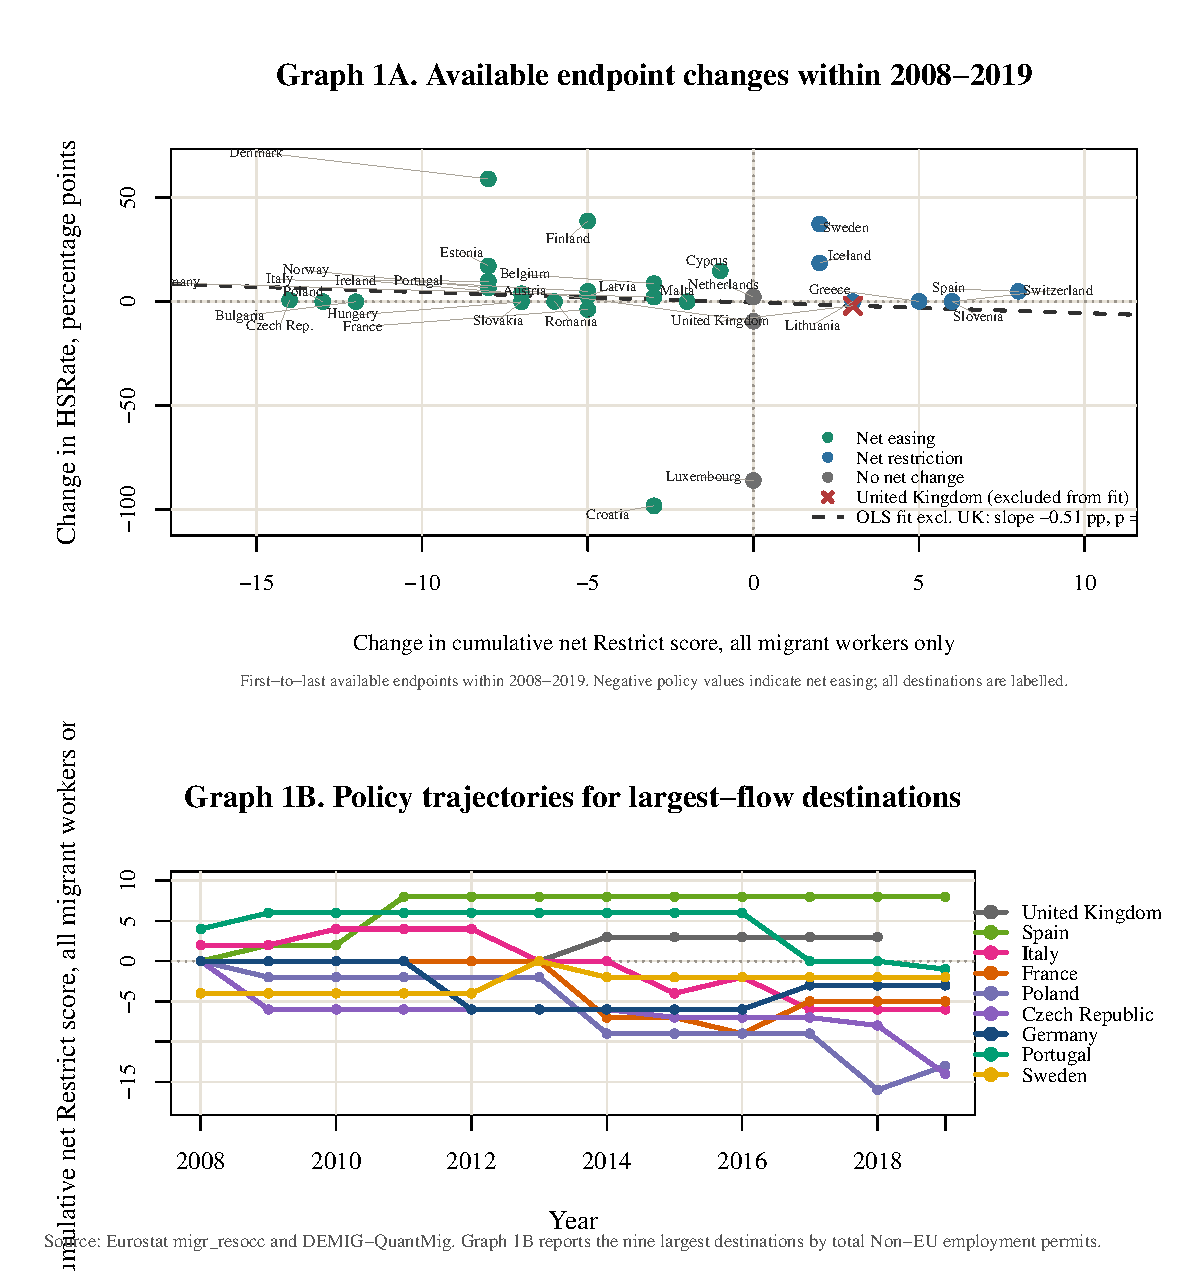
\includegraphics[width=\linewidth,height=0.79\textheight,keepaspectratio]{figures/graph1_outcomes_and_policy.pdf}
\end{center}

\captionof{figure}[Descriptive policy change and HSRate]{Descriptive relationship between cumulative net policy-change score and HSRate within 2008--2019. Graph 1A shows each destination's first-to-last available endpoint change within the window; seven series do not contain both exact boundary years. Graph 1B reports cumulative policy paths for the nine largest destinations by total Non-EU employment permits in Eurostat over 2008--2019. The United Kingdom is marked separately because of Brexit. Graph 1A covers 31 descriptive series, whereas the main controlled regressions retain 30 destination clusters after the lagged-control complete-case filter.}\label{graph:descriptive}

The main takeaway from Graph 1A is deliberately modest. The descriptive
scatter does not visually confirm a simple relationship in which
restriction mechanically increases HSRate: most destinations sit on the
net-easing side, HSRate changes are heterogeneous, and the endpoint
slope is not statistically significant. This is why the formal
fixed-effects models, rather than Graph 1, carry the empirical test.

Graph 1B shows the nine destinations with the largest observed Non-EU
employment-permit flows. Twenty of the 31 available endpoint series move
toward net liberalization, and about 62 percent of retained
all-migrant-worker events are coded as less restrictive. The
fixed-effects models, rather than this descriptive figure, test whether
within-destination policy change is associated with HSRate.

Using each series' first and last available observations within the
window, HSRate rises in 22 destinations, is unchanged in three, and falls
in six. Belgium, Croatia, Iceland, Luxembourg, the Netherlands,
Switzerland, and the United Kingdom use shorter endpoint windows because
one or both exact boundary years are unavailable. The descriptive
pattern is affected by small denominators and institutional breaks,
including Brexit, so it is not used as evidence for the main claim.

\section{7. Results}\label{results}

\subsection{7.1 Aggregate country-year
results}\label{aggregate-country-year-results}

The aggregate destination-year models are reported first as a benchmark before
origin-side pressures are absorbed. They do not show a detectable composition
association. One possible reason is that high-skilled migration also depends
on origin conditions, networks, labor-market opportunities, and the relative
attractiveness of other destinations, none of which is represented fully in a
destination-year model. Imprecision is another possibility, so the aggregate
null results are not themselves proof that origin-side factors explain the
difference.

In the full aggregate model, the all-migrant-worker cumulative coefficient is
beta = 0.002296 with cluster-robust SE = 0.001925 (t = 1.19, p = 0.243, N =
280, G = 30). The annual policy-flow estimate is also not significant (beta =
0.000796, SE = 0.002334, p = 0.736), and neither is the aggregate log
high-skilled-count outcome (beta = 0.022422, SE = 0.027276, p = 0.418). The
aggregate evidence therefore provides no support for a composition or
high-skilled-count association under the preferred policy definition. The main
test is the bilateral specification in Section 7.2.

\Needspace{7\baselineskip}\captionof{table}[Aggregate country-year regression results]{Aggregate country-year regression results. Outcome: high-skilled share, except M4 (log high-skilled permit count).}\label{tab:aggregate-results}

\begin{center}
\scriptsize
\setlength{\tabcolsep}{3.2pt}
\renewcommand{\arraystretch}{1.00}
\begin{tabularx}{\linewidth}{@{}>{\RaggedRight\arraybackslash}X*{6}{Y}@{}}
\toprule
 & \textbf{M0} & \textbf{M1} & \textbf{M2} & \textbf{M3} & \textbf{M4} & \makecell{\textbf{Annual}\\\textbf{flow}} \\
\midrule
\multicolumn{7}{@{}l}{\textit{Policy coefficient}} \\
Lagged all-migrant-worker policy score
  & -0.000163 & 0.000748 & 0.002102 & 0.002296 & 0.022422 & 0.000796 \\
\textit{Cluster-robust SE}
  & (0.002118) & (0.001890) & (0.001791) & (0.001925) & (0.027276) & (0.002334) \\
Exact p-value
  & 0.939 & 0.695 & 0.250 & 0.243 & 0.418 & 0.736 \\
\addlinespace[1pt]
\multicolumn{7}{@{}l}{\textit{Specification}} \\
Outcome
  & HS share & HS share & HS share & HS share & \makecell{Log HS\\count} & HS share \\
Skill-target policy controls
  & \no & \yes & \yes & \yes & \yes & \yes \\
Lagged permit scale
  & \no & \no & \yes & \yes & \yes & \yes \\
Destination macro controls
  & \no & \no & \no & \yes & \yes & \yes \\
\midrule
Observations
  & 341 & 341 & 312 & 280 & 280 & 280 \\
Destination clusters
  & 31 & 31 & 31 & 30 & 30 & 30 \\
\bottomrule
\end{tabularx}
\end{center}

\TableNote{All models include destination and year fixed effects. M0 and
M1 include 2008--2019 because they do not require lagged permit scale.
M2-M4 begin in 2009 because the 2008 outcome has no 2007 permit value
from which to construct that control; missing unemployment further
reduces the full-control sample. All columns apply the minimum current
employment-permit denominator of 30. The progressive coefficients are
therefore not estimated on an identical sample. In all regression
tables, N denotes the observations retained after the outcome, lags,
controls, and fixed effects are jointly available; G denotes destination
clusters. *** $p<0.01$, ** $p<0.05$, * $p<0.10$.}

Table 6 shows that none of the aggregate coefficients reaches
five-percent significance as controls are added. The thesis therefore
bases its main claim on the bilateral model, where origin-year fixed
effects absorb migration pressures that are lost in aggregation.

\subsection{7.2 Preferred bilateral origin-year fixed-effects
result}\label{preferred-bilateral-origin-year-fixed-effects-result}

The bilateral specification is the main test of the Section 3
prediction. It uses the all-migrant-worker-only cumulative measure,
origin-year fixed effects, and permit-denominator weights. These choices
address two weaknesses of the aggregate model: unobserved origin-side
conditions and noisy shares in small permit cells.

\Needspace{7\baselineskip}\captionof{table}{Preferred bilateral specification and comparison models.}\label{tab:bilateral-results}

\begin{center}
\scriptsize
\setlength{\tabcolsep}{3.4pt}
\renewcommand{\arraystretch}{1.00}
\begin{tabularx}{\linewidth}{@{}>{\RaggedRight\arraybackslash}X*{4}{Y}@{}}
\toprule
 & \makecell{\textbf{Preferred}\\\textbf{weighted}} &
   \makecell{\textbf{Unweighted}\\\textbf{comparison}} &
   \makecell{\textbf{Weighted}\\\textbf{corridor FE}} &
   \makecell{\textbf{Annual}\\\textbf{policy flow}} \\
\midrule
\multicolumn{5}{@{}l}{\textit{Coefficients}} \\
Lagged cumulative all-migrant-worker score
  & 0.006516*** & 0.004587** & 0.005495*** & \NA \\
\textit{Cluster-robust SE}
  & (0.001612) & (0.001850) & (0.001565) & \NA \\
Exact p-value
  & $<$0.001 & 0.019 & 0.0015 & \NA \\
Lagged annual all-migrant-worker policy flow
  & \NA & \NA & \NA & 0.000407 \\
\textit{Cluster-robust SE}
  & \NA & \NA & \NA & (0.001935) \\
Exact p-value
  & \NA & \NA & \NA & 0.835 \\
\addlinespace[1pt]
\multicolumn{5}{@{}l}{\textit{Specification}} \\
Skill-target policy paths
  & Cumulative & Cumulative & Cumulative & Annual \\
Permit-denominator weights
  & \yes & \no & \yes & \no \\
Destination fixed effects
  & \yes & \yes & \no & \yes \\
Origin-destination corridor fixed effects
  & \no & \no & \yes & \no \\
\midrule
Observations
  & 5,608 & 5,608 & 5,608 & 5,608 \\
Destination clusters
  & 30 & 30 & 30 & 30 \\
\bottomrule
\end{tabularx}
\end{center}

\TableNote{Outcome: bilateral high-skilled share of
employment-related permits. All models include origin-year fixed
effects, lagged bilateral permit scale, lagged destination unemployment,
lagged destination GDP growth, and the corresponding high- and low-skill
policy paths; standard errors cluster by destination. The preferred,
unweighted, and annual-flow models use destination fixed effects, while
the corridor model replaces them with origin-destination fixed effects.
The preferred and corridor models use employment-permit-denominator
weights. All columns retain cells with at least 30 current employment
permits. The preferred model's high- and low-skill policy-control
coefficients are reported in Appendix Table A.2.}

The preferred weighted coefficient is beta = 0.006516 with cluster-robust SE =
0.001612 (t = 4.04, p $<$ 0.001, N = 5,608 origin-destination-year cells across
G = 30 destinations). The wild-cluster bootstrap p-value is 0.007, so the
result remains significant after the few-cluster correction. A one-unit
increase in lagged cumulative net policy change for all-migrant-worker reforms
is associated with a 0.65-percentage-point increase in HSRate, conditional on
destination and origin-year fixed effects, lagged bilateral permit scale,
destination macro controls, and the two skill-targeted policy controls. Those
high-skilled policy control is imprecisely estimated (beta = 0.001423, p =
0.446). The low-skilled policy control is negative and marginal at ten percent
(beta = -0.008571, p = 0.085), so it is not treated as main evidence.

Scaling the estimate by event magnitude makes its size easier to interpret. A
Mid-level restrictive reform contributes three cumulative units, corresponding
to a 1.95-percentage-point higher HSRate the following year. A Major reform
contributes four units, corresponding to 2.61 percentage points. Relative to
the bilateral-sample mean HSRate of 21.0 percent, the Major-reform calculation
is about 12.4 percent of the mean. The comparable full-control aggregate
coefficient is smaller and imprecise (beta = 0.002296, p = 0.243); its
four-unit calculation is about 0.92 percentage points and is not statistically
distinguishable from zero.

The alternative bilateral models clarify which design choices matter. The
unweighted controlled estimate remains positive (beta = 0.004587, SE =
0.001850, p = 0.019), but its wild-cluster bootstrap p-value is 0.079. After
the few-cluster correction, the strongest evidence therefore comes from the
denominator-weighted estimator chosen in advance. The weighted
corridor-fixed-effects estimate is also positive and significant (beta =
0.005495, SE = 0.001565, p = 0.0015; bootstrap p = 0.0045), so the
retained-sample result does not depend only on stable corridor differences.

Section 8 shows that the weighted result also survives removal of the EMP
$\geq 30$ cutoff, although the unweighted no-cutoff estimate is imprecise. By
contrast, the bilateral annual policy-flow coefficient is not significant
(beta = 0.000407, p = 0.835). The preferred finding is therefore a cumulative
net-policy-change association, not evidence of a short-run response to newly
adopted annual events.

\subsection{7.3 Interpretation of the significant and non-significant
findings}\label{interpretation-of-the-significant-and-non-significant-findings}

The results show a positive composition association and a positive measured
high-skilled permit count, but no statistically detectable change in the
bilateral total employment-permit count. In the preferred denominator-weighted
bilateral model, the cumulative net policy-change measure is positively
associated with the high-skilled share (beta = 0.006516, p $<$ 0.001, N = 5,608;
bootstrap p = 0.007), consistent with the prediction in Section 3. The
aggregate cumulative and annual-flow share models are not significant. In the
bilateral PPML comparison, the measured high-skilled count is positive and
significant, while the total employment-permit count is not. The evidence
therefore points to a change in composition within the retained corridor
sample, not to a proven increase in overall employment-permit volume.

\Needspace{14\baselineskip}\captionof{table}{PPML estimates for bilateral permit-count outcomes.}\label{tab:ppml-results}

\begin{center}
\footnotesize
\setlength{\tabcolsep}{5pt}
\renewcommand{\arraystretch}{1.08}
\begin{tabularx}{0.90\linewidth}{@{}>{\RaggedRight\arraybackslash}X*{2}{Y}@{}}
\toprule
 & \makecell{\textbf{(1)}\\\textbf{High-skilled}\\\textbf{permit count}}
 & \makecell{\textbf{(2)}\\\textbf{Total employment-}\\\textbf{permit count}} \\
\midrule
\multicolumn{3}{@{}l}{\textit{Policy coefficient}} \\
Lagged cumulative all-migrant-worker score
  & 0.045536*** & -0.025527 \\
\textit{Cluster-robust SE}
  & (0.012895) & (0.017454) \\
Exact p-value
  & 0.0016 & 0.1543 \\
\addlinespace[2pt]
\multicolumn{3}{@{}l}{\textit{Specification}} \\
High-skilled policy control
  & \yes & \yes \\
Low-skilled policy control
  & \yes & \yes \\
Destination macro controls
  & \yes & \yes \\
Destination fixed effects
  & \yes & \yes \\
Origin-year fixed effects
  & \yes & \yes \\
Lagged PermitScale control
  & \no & \no \\
Permit-denominator weights
  & \no & \no \\
\midrule
Observations
  & 5,219 & 5,608 \\
Destination clusters
  & 27 & 30 \\
\bottomrule
\end{tabularx}
\end{center}

\TableNote{Poisson Pseudo-Maximum-Likelihood estimates corresponding to Equation (4), estimated on the corridors retained by the main EMP $\geq 30$ share-sample rule. The dependent variable is HSNumber in column (1) and the total employment-permit count, EMP, in column (2). Both models include lagged destination unemployment and GDP growth. For column (1), separated destination and origin-year fixed-effect groups with all-zero high-skilled counts are removed before estimation; this reduces the sample from 5,608 cells and 30 clusters to 5,219 cells and 27 clusters. Standard errors clustered by destination are reported in parentheses. Coefficients are semi-elasticities; the exact percentage change associated with one Restrict unit is \(100[\exp(\beta)-1]\). *** \(p<0.01\), ** \(p<0.05\), * \(p<0.10\).}

Column (1) of Table~\ref{tab:ppml-results} is positive and significant at
the one-percent level: one additional Restrict unit is associated with
an exact estimated increase of about 4.66 percent in HSNumber. Column (2)
is negative but imprecise; its exact point estimate is about -2.52 percent.
Because separation pruning gives the
two columns different effective samples, their coefficients are not
subtracted as a formal decomposition. Read separately, they indicate a
higher high-skilled count without a statistically detectable change in
the total employment-permit count. This is consistent with the positive
HSRate result, but it still does not identify the causal count response
to a particular reform or the unobserved lower-skilled count directly.

The positive HSNumber estimate in Table~\ref{tab:ppml-results} should not
be interpreted as evidence that general restrictions attract additional
skilled migrants. HSNumber counts first permits recorded under the
administrative highly-skilled-worker and researcher categories rather
than entrants' underlying skills. When broader employment rules tighten,
some recruitment may be redirected from other employment routes into
dedicated high-skilled categories, increasing measured HSNumber without
increasing total skilled arrivals. Because the data do not follow
individuals across routes, this mechanism cannot be tested directly.
Appendix Table~\ref{tab:app-tier1} reports exploratory diagnostics: only
the highly-skilled-worker category has a significant positive
coefficient; the non-high-skilled employment-permit estimate is negative but
imprecise; the following year's policy flow is insignificant; and adding
2020 attenuates but does not overturn the preferred result. However, the category
models use different samples, and the preferred share estimate becomes
smaller and insignificant when destination-specific trends are added.
These diagnostics are compatible with, but do not establish,
reallocation.

This interpretation is also consistent with the contrast between
aggregate and bilateral specifications. Under the same design,
the aggregate cumulative all-migrant-worker model with high-skilled and
low-skilled policy controls is not significant (\(\beta =\) 0.002296, p
= 0.243, N = 280), and the aggregate annual-flow version is also not
significant (\(\beta =\) 0.000796, p = 0.736, N = 280). The
denominator-weighted bilateral model, however, remains significant after
controlling for skilled/high-skilled and low-skilled target-group policy
paths (\(\beta =\) 0.006516, p $<$ 0.001, N = 5,608). The substantive
story is therefore narrower and more precise than a simple aggregate
reading would suggest. General restrictions are associated with
composition when the specification absorbs origin-year migration
pressures, accounts for noisy small-denominator cells, and separates
broad all-migrant-worker reforms from targeted skill-selective reforms.

\section{8. Robustness, Sensitivity, and Diagnostic
Checks}\label{robustness-sensitivity-and-diagnostic-checks}

Section 8 brings the robustness, sensitivity, and diagnostic evidence together
in Table~\ref{tab:robustness}. Panel A modifies the preferred
denominator-weighted bilateral model, while Panel B reports two aggregate EU27
placebo comparisons. Because the panels answer different questions, their
coefficients should not be interpreted as estimates from one common model.

The overall pattern is mixed but informative. The preferred result survives
reintroducing 2020, removing the minimum-cell cutoff, using the
all-first-permits denominator, replacing unemployment with no-UK ILOSTAT data,
narrowing the policy measure to core labor-entry or work-visa tools, using
prior-year weights, and adding EU-directive windows. The origin-income
estimates remain heterogeneous, the UK-inclusive model and aggregate placebo
coefficients are not significant, and destination-specific trends
substantially weaken the estimate. Every leave-one-destination-out coefficient
remains positive and significant at five percent.

Within Panel B, the EU27 placebo is constructed only as an aggregate
diagnostic. It sums permit counts across the fixed EU27-2020 citizenship
composition, excluding the reporting destination\textquotesingle s own
citizenship, and reconstructs HSNumber, HSRate, and PermitScale from
those EU27 permit flows. The cumulative and annual-flow specifications
then use the same policy variables, macroeconomic controls, and fixed
effects as their Non-EU aggregate counterparts. Because EU citizens
generally enter under free-movement rights rather than the national
labor-migration rules measured by Restrict, the expected placebo
coefficient is close to zero. Sparse and selective EU permit reporting,
accession timing, and transitional restrictions nevertheless make this
a limited diagnostic rather than a clean untreated comparison group.

\Needspace{7\baselineskip}\captionof{table}{Robustness, sensitivity, and diagnostic checks.}\label{tab:robustness}

{\def\LTcaptype{none} % do not increment counter
\setlength{\LTpost}{0pt}
\begin{longtable}[]{@{}
  L{(\linewidth - 8\tabcolsep) * \real{0.20}}
  L{(\linewidth - 8\tabcolsep) * \real{0.39}}
  C{(\linewidth - 8\tabcolsep) * \real{0.13}}
  C{(\linewidth - 8\tabcolsep) * \real{0.09}}
  L{(\linewidth - 8\tabcolsep) * \real{0.19}}@{}}
\toprule\noalign{}
\textbf{Design / check} & \textbf{Change relative to the reference model} &
\(\boldsymbol{\beta}\) & \textbf{p} & \textbf{Inference} \\
\midrule\noalign{}
\endhead
\bottomrule\noalign{}
\endlastfoot
\multicolumn{5}{@{}l}{\textbf{Panel A. Robustness and sensitivity checks}} \\
\addlinespace[2pt]
Bilateral: include 2020 pandemic year & Extends the baseline outcome window from 2008--2019 to 2008--2020 & 0.005446*** & 0.004 & Significant; bootstrap p = 0.024 \\
Bilateral: no minimum-cell cutoff & Retains every positive employment-permit denominator & 0.005978*** & $<$0.001 & Significant; not created by cutoff \\
Bilateral: all-first-permits denominator & Replaces the employment-permit denominator with all first residence permits & 0.000958*** & 0.004 & Significant; survives broader denominator \\
Bilateral: ILOSTAT, no UK & Replaces Eurostat unemployment with ILOSTAT & 0.005547*** & $<$0.001 & Significant; survives source change \\
Bilateral: ILOSTAT, with UK & Adds the United Kingdom using ILOSTAT unemployment & 0.000883 & 0.774 & Not significant \\
Bilateral: core labor-entry measure & Restricts the policy index to core labor-entry and administrative tools & 0.004389** & 0.015 & Positive and significant \\
Bilateral: work-visa tool only & Restricts the policy index to work-visa and work-permit events & 0.008190*** & $<$0.001 & Significant; larger estimate \\
Bilateral: origin-income strata & Re-estimates the preferred model by World Bank FY2020 origin-income group & See text & Sig. & Positive for H/UM/LM; negative for L \\
Bilateral: EU directive windows & Adds four destination-year directive-window controls where legally applicable & 0.006587*** & $<$0.001 & Preferred coefficient remains stable \\
Bilateral: prior-year denominator weights & Replaces the current-year precision weight with the previous year's employment-permit denominator & 0.006858*** & $<$0.001 & Significant; bootstrap p = 0.0025 \\
Bilateral: leave-one-destination-out & Re-estimates the preferred model omitting each of the 30 destinations in turn & 0.0039 to 0.0073 & See text & Positive and significant in all 30 runs \\
\addlinespace[3pt]
\multicolumn{5}{@{}l}{\textbf{Panel B. Aggregate EU27 placebo diagnostics}} \\
\addlinespace[2pt]
Non-EU group, cumulative score & Aggregate treated-group benchmark & 0.002296 & 0.243 & Not significant (N=280; G=30) \\
EU27 placebo, cumulative score & Applies the aggregate model to the fixed EU27-2020 citizenship group & 0.021964 & 0.217 & Not significant; small sample (N=38; G=13) \\
Non-EU group, annual policy flow & Tests newly adopted policy changes against the following year's outcome & 0.000796 & 0.736 & Not significant (N=280; G=30) \\
EU27 placebo, annual policy flow & Repeats the annual-flow test for the fixed EU27-2020 citizenship group & 0.003328 & 0.720 & Not significant; small sample (N=38; G=13) \\
\end{longtable}
}

\LongTableNote{*** $p<0.01$, ** $p<0.05$, * $p<0.10$. Panel A changes a model,
outcome, sample, data source, or policy definition within the preferred bilateral
framework; the no-cutoff row retains every positive denominator. Panel B provides limited aggregate falsification diagnostics. Bilateral and aggregate coefficients are not directly
comparable because the designs, fixed effects, weighting, outcomes, and
samples differ. The preferred result remains the denominator-weighted bilateral
HSRate specification in Table 7.}

The first robustness check reintroduces the pandemic year. Extending the
outcome window from 2008--2019 to 2008--2020 reduces the preferred coefficient
from 0.006516 to 0.005446, but the extended-window estimate remains positive
and significant (SE = 0.001716, p = 0.004, N = 6,301; wild-cluster bootstrap p
= 0.024). The exclusion of 2020 therefore strengthens the baseline estimate
but does not create its sign or statistical significance.

The next sensitivity removes the minimum-cell cutoff while retaining
the preferred denominator weights. The coefficient remains positive and
significant (\(\beta =\) 0.005978, p $<$ 0.001, N = 21,187), so the weighted
result is not created by dropping corridors below 30 permits. The
unweighted no-cutoff comparison is positive but imprecise (\(\beta =\)
0.002565, p = 0.283). This contrast shows that the preferred evidence is
robust to the cutoff but still depends on the precision weighting that
defines the estimand.

A related sensitivity check splits the cumulative net score into separate
restrictive and liberalising stocks instead of netting them. In the unweighted
bilateral design with skill-target controls, the liberalising stock is negative
and significant (beta = -0.006893, p = 0.005), while the restrictive stock
alone is imprecise (p = 0.551). Because about 62 percent of retained
all-migrant-worker events are liberalisations, the identifying variation comes
mainly from easing episodes: opening the general channel is associated with a
lower high-skilled share. This is the mirror image of the restriction reading
and is consistent with the entry-channel mechanism in Section 3.

Robustness 1 tests whether the preferred result depends on the
employment-permit denominator. It keeps highly skilled worker and researcher
permits in the numerator but divides them by all first residence permits in
the same cell, including family, education, employment, and other reasons.
Under the preferred policy specification, the weighted bilateral coefficient
remains positive and significant (beta = 0.000958, p = 0.004, N = 4,735). The
corridor-FE variant is also significant (beta = 0.000975, p = 0.031), as is
the version retaining the original employment-permit scale control (beta =
0.001015, p = 0.001, N = 5,608).

The result is therefore not only a mechanical feature of the employment-permit
denominator. This remains a secondary check, however, because the broader
denominator includes family, education, and other permit channels that
labor-migration policy does not directly target.

Robustness 2 (core labor-entry subset) asks whether the result depends
on the exact set of DEMIG-QuantMig policy tools retained in the
preferred Restrict measure. The core labor-entry subset retains only the
policy tools that directly affect the employer-permit entry decision:
work visa/permit rules, quota/target, entry visa/stay permit, employer
liabilities, and other sanctions tied to non-compliance. It excludes
free mobility rights or agreements, action plans and strategy reports,
integration programs, and general access-to-rights categories. These
excluded tools are part of the DEMIG-QuantMig Legal entry and stay area
but do not directly govern who is admitted under the general work-permit
channel. After adding the high-skilled and low-skilled target-group
policy controls, the core-subset estimate remains positive and significant
(\(\beta =\) 0.004389, p = 0.015). The result is therefore not confined to
the broader all-tools definition, although the subset still combines several
distinct legal instruments.

Panel B of Table~\ref{tab:robustness} contains the aggregate EU27
placebo diagnostics. They do not test the robustness of the preferred
bilateral estimator. Instead, they ask whether the aggregate policy
association also appears for a group that is less directly exposed to
national labor-migration rules.

The cumulative EU27 placebo is positive but not statistically
significant (0.021964, p = 0.217), while the aggregate Non-EU
counterpart is also small and imprecise (M3: 0.002296, p = 0.243). Because
the EU27 estimate is based on only 38 observations and 13 destination
clusters, it is too imprecise to establish a clear alternative
explanation by itself. The fixed EU27-2020
composition also spans Croatia's accession and temporary labor-market
restrictions, so it is not a clean untreated group. This aggregate
placebo does not directly validate the preferred bilateral estimate, but
it also does not reproduce a statistically significant aggregate policy
association for the less-exposed group.

The annual-flow EU27 placebo is also not significant
(\(\beta =\) 0.003328, p = 0.720), again on only 38
observations and 13 clusters. The thesis therefore treats both EU27
results as limited diagnostics rather than as strong identification
tests. A bilateral
version of the EU27 placebo, which would have been the closest mirror of
the preferred denominator-weighted bilateral design, is not run because
EU-origin residence-permit cells are too sparse and selective to provide
a comparable bilateral outcome: EU free movers generally do not require
the permits measured by migr\_resocc. Although the raw extract contains
individual EU citizenship rows, treating those permit observations as a
bilateral migration-flow panel would not mirror the Non-EU outcome. The
aggregate EU27 check is therefore retained only as a limited diagnostic.

Robustness 3 replaces Eurostat unemployment with World Bank indicator
SL.UEM.TOTL.ZS, the modeled ILO unemployment estimate sourced from
ILOSTAT (World Bank 2026), and estimates no-UK and UK-inclusive variants. The main
Eurostat sample excludes the United Kingdom because the Eurostat control
extract used here contains no UK unemployment observations for the
estimation window; Brexit is also not fully represented as a single
change in the cumulative policy score.

The weighted preferred result is robust to replacing Eurostat
unemployment with ILOSTAT when the United Kingdom remains excluded. The
Eurostat no-UK weighted estimate is \(\beta =\) 0.006516 with SE =
0.001612 (p $<$ 0.001, N = 5,608, G = 30). The ILOSTAT no-UK weighted
estimate is \(\beta =\) 0.005547 with SE = 0.001258 (p $<$ 0.001, N =
5,962, G = 30). The point estimate is slightly smaller but remains
significant at the five-percent level. When the United Kingdom is added
through ILOSTAT, however, the coefficient falls to \(\beta =\) 0.000883
with SE = 0.003041 (p = 0.774, N = 6,638, G = 31). This supports the
same interpretation as before: the main weighted result is not driven by
the Eurostat unemployment source, but it is conditional on excluding a
destination whose post-2016 migration-policy regime is not well
represented by the cumulative net policy-change measure.

The UK exercise is a limitation rather than proof that UK inclusion is
inappropriate: the preferred result is conditional on the no-UK sample,
and the Brexit-era measurement mismatch is a plausible explanation for
the difference.

Robustness 4 examines heterogeneity by origin income using the World
Bank FY2020 income classification, published in 2019 and based on 2018
Atlas-method GNI per capita (World Bank Data Team 2019). Under the
controlled model, the association remains positive and
significant for high-income origins (\(\beta =\) 0.016784, p = 0.003),
upper-middle-income origins (\(\beta =\) 0.004139, p = 0.014), and
lower-middle-income origins (\(\beta =\) 0.006739, p = 0.001). The
low-income-origin estimate is negative but only marginal at ten percent
(\(\beta = -0.002422\), p = 0.083), and this stratum is smaller (N =
347, G = 19), so it is not treated as a statistically established reversal.
It should be
interpreted cautiously. Overall, the income-stratified results are
heterogeneous rather than a uniform confirmation of the
entry-channel-elasticity mechanism: the association is positive for
high-, upper-middle-, and lower-middle-income origins but reverses sign
for low-income origins. This pattern may reflect differences in access
to dedicated routes, credential recognition, financial constraints, or
the composition of origin-destination corridors, none of which is
measured directly in the present design. The heterogeneity analysis
should therefore be read as qualifying the proposed mechanism and
identifying a direction for future research, rather than as a direct
test of why the composition response differs across origin-income
groups.

Robustness 5 narrows Restrict to the Work visa/permit tool, the instrument
most directly tied to the general employment-permit channel. The same
denominator-weighted bilateral model is re-estimated on N = 5,608 cells and G
= 30 destinations, with destination and origin-year fixed effects,
skill-targeted policy controls, lagged economic controls, and denominator
weights.

The work-visa-only coefficient is beta = 0.008190 with cluster-robust SE =
0.001620 (t = 5.05, p $<$ 0.001; wild-cluster bootstrap p = 0.0048), moderately
larger than the all-tools estimate of 0.006516. This is consistent with the proposed mechanism because the
measure is narrowed to the tool most directly governing the general
work-permit track.

The check does not isolate that mechanism cleanly. Work visa/permit is also
common among skilled/high-skilled-targeted reforms, so its changes may
correlate with policies that directly affect high-skilled entry. The
skill-targeted controls reduce but cannot eliminate that overlap. The result
is therefore corroborating evidence, while the broader all-tools measure
remains preferred because it matches the policy-area definition in Section
6.2.

Robustness 6 asks whether common EU directive windows account for the
preferred association. It adds timing indicators for the Blue Card, Single
Permit, Intra-Corporate Transferee, and Students and Researchers directives.
Indicators are activated only for participating destinations in the relevant
years: Croatia enters from 2013, while Denmark and Ireland are excluded where
they do not participate.

A single combined applicable-window indicator gives beta = 0.006518 with SE =
0.001619 (p $<$ 0.001). Adding the four directive indicators separately gives
beta = 0.006587 with SE = 0.001581 (p $<$ 0.001). Both estimates are close to
the preferred coefficient of 0.006516, and none of the directive indicators is
individually significant at the five-percent level. The result is therefore
not explained by these measured directive windows, although they are coarse
timing proxies rather than reform-specific causal estimates. Graph 3 reports
the directive coefficients and the adoption and transposition windows used to
construct them.

\clearpage
A prior-year-weight check addresses the concern that the current denominator
may respond to the same policy environment used to explain HSRate. Replacing
it with the previous year's employment-permit denominator leaves the estimate
essentially unchanged and slightly more precise (beta = 0.006858, SE =
0.001502, p $<$ 0.001; wild-cluster bootstrap p = 0.0025, N = 5,540). Same-period
weighting therefore does not create the preferred result, although the lagged
denominator can still reflect earlier policy history.

A leave-one-destination-out check then omits each of the 30 destinations in
turn. The coefficient remains positive and significant at five percent in all
30 runs, ranging from 0.003884 to 0.007334. France is the most influential
omission: excluding it gives beta = 0.003884 with p = 0.029. No single
destination therefore drives either the sign or conventional five-percent
significance of the baseline result.

Graph 2 summarizes the main estimates, robustness checks, and placebo
diagnostics; bars show 95-percent confidence intervals and the dashed
line marks zero.

\begin{center}
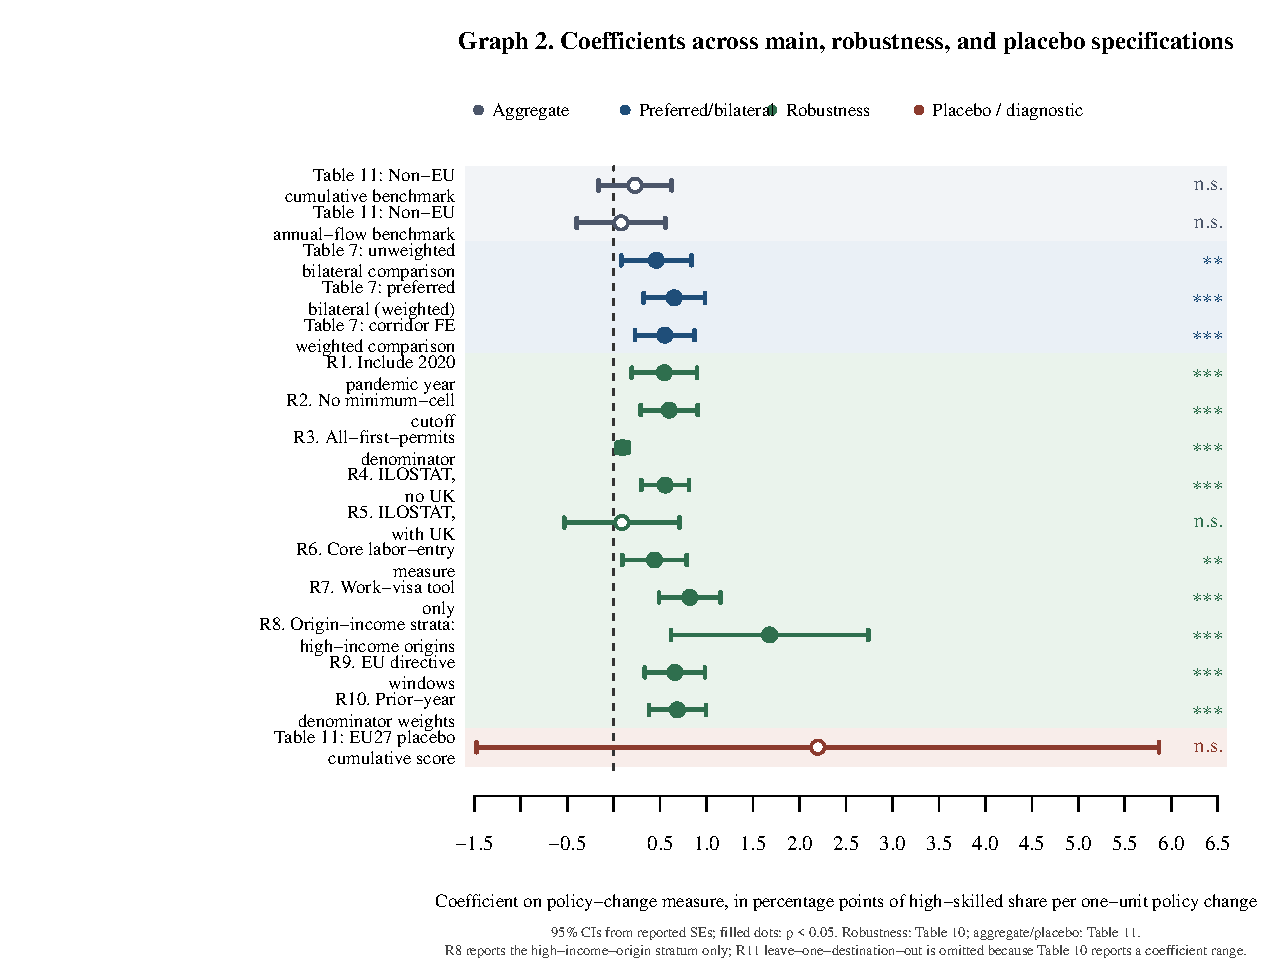
\includegraphics[width=\linewidth,height=0.76\textheight,keepaspectratio]{figures/graph2_robustness_coefficient_plot.pdf}
\end{center}

\captionof{figure}[Coefficient estimates across specifications]{Coefficient estimates across specifications. Coefficients are in percentage-point units; bars show 95-percent confidence intervals and the dashed line marks zero. Preferred bilateral and robustness rows report the all-migrant-worker coefficient with skill-targeted policy controls where applicable. The EU27 row is an aggregate placebo; models and samples differ across rows.}\label{graph:coefficients}

Graph 2 reinforces the tables: evidence is strongest in the controlled
bilateral specifications. The aggregate estimates, UK-inclusive check, and
EU27 placebo are not significant. The 2020-inclusive, no-cutoff, core-tool,
prior-year-weight, all-first-permits, work-visa-only, and EU-directive checks
remain significant.

\begin{center}
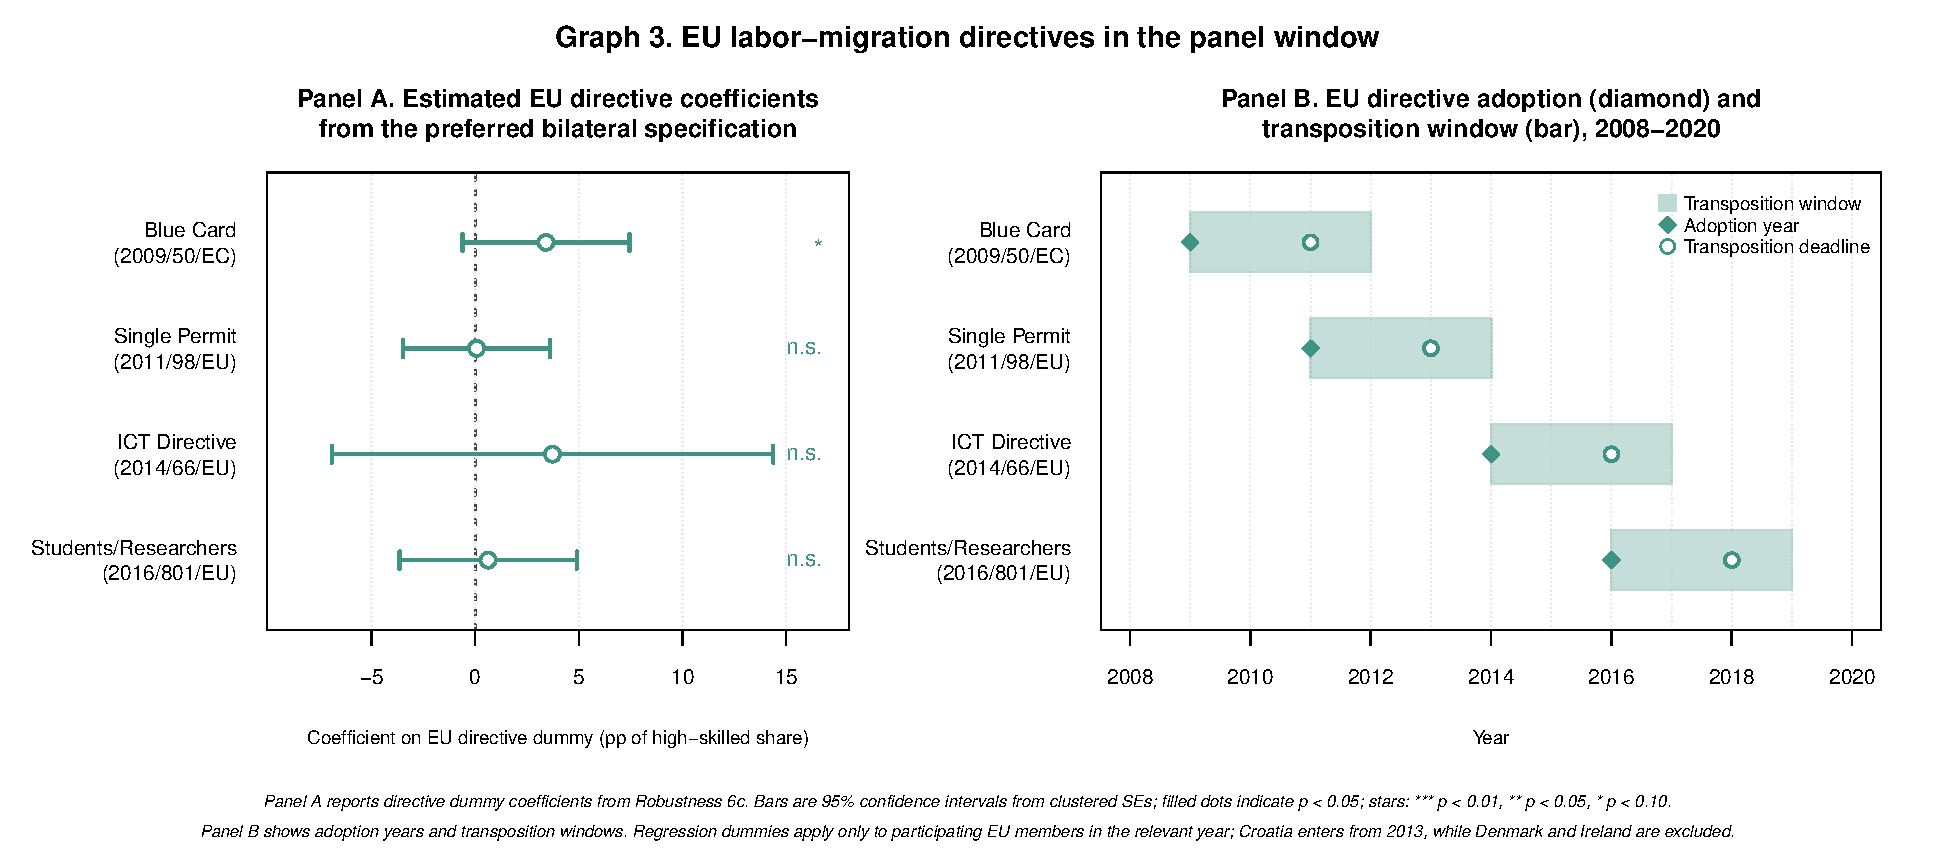
\includegraphics[width=\linewidth,height=0.72\textheight,keepaspectratio]{figures/graph3_eu_directives.pdf}
\end{center}

\captionof{figure}[EU labor-migration directives in the panel window]{EU labor-migration directives in the panel window. Panel A reports the coefficient of each EU directive dummy in the preferred denominator-weighted bilateral specification (Robustness 6, specification c), in percentage points of the high-skilled share, with 95-percent cluster-robust confidence intervals. Filled dots indicate $p<0.05$. The regression dummies apply only to participating EU members in the relevant year: Croatia enters from 2013, while Denmark and Ireland are excluded. Panel B shows each directive's adoption year (diamond), transposition window (shaded bar), and deadline (open circle) between 2008 and 2019.}\label{graph:directives}

Panel A shows that none of the four directive-window coefficients is
statistically significant. More importantly, the preferred Restrict
coefficient remains positive and significant (\(\beta =\) 0.006587, p $<$
0.001), indicating that the main association is not accounted for by
these measured directive windows. Panel B shows the adoption and
transposition periods used to construct the controls; these windows are
coarse timing proxies rather than directive-specific causal estimates.

\clearpage
\begin{center}
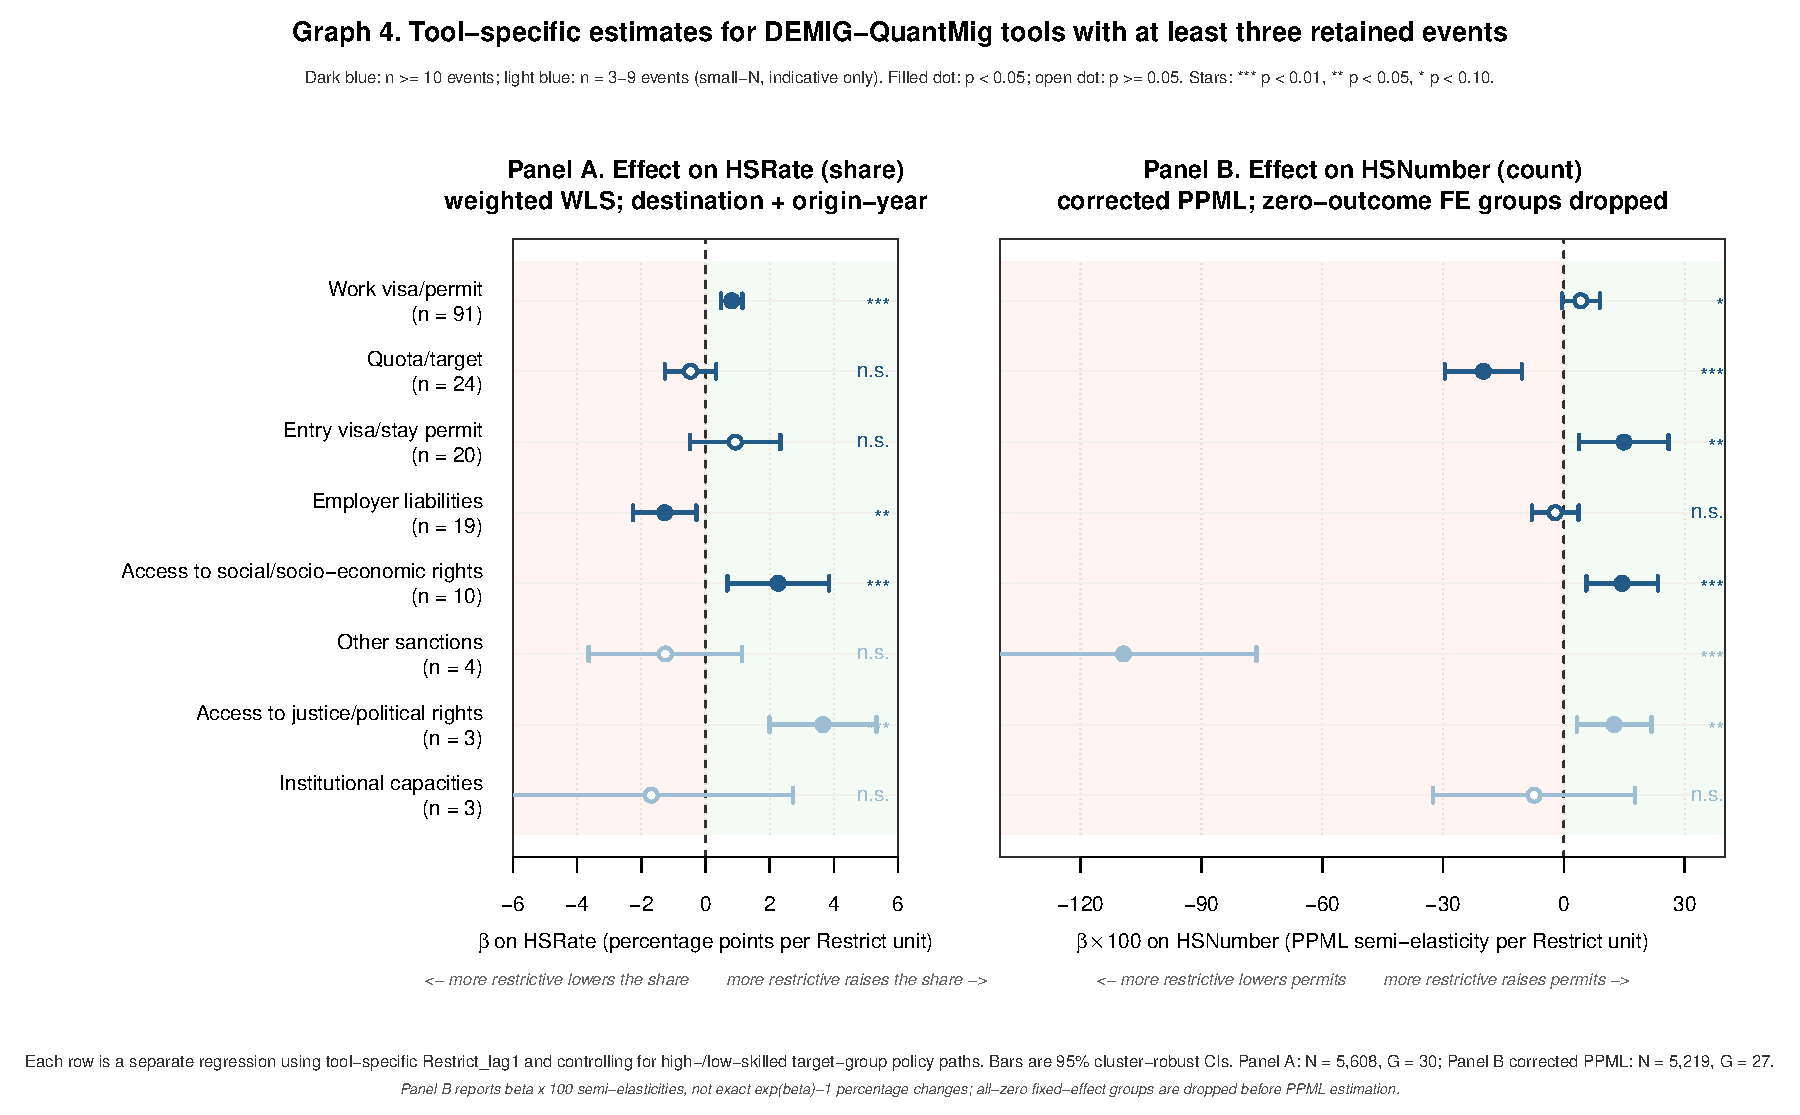
\includegraphics[width=\linewidth,height=0.74\textheight,keepaspectratio]{figures/graph4_tool_specific_corrected.pdf}
\end{center}

\captionof{figure}[Tool-specific policy estimates]{Tool-specific estimates for DEMIG-QuantMig policy tools with at least three retained events: each row reports the tool's separate association with HSRate and HSNumber.}\label{graph:tools}

Graph 4 is a tool-specific diagnostic, not a decomposition of the
preferred coefficient. Each row re-estimates the preferred specification
using one policy tool; the PPML count panel drops all-zero fixed-effect
groups (N = 5,219; G = 27).

Work visa/permit, the largest tool category, is share-positive (0.82
percentage points; p $<$ 0.001) and broadly consistent with the
work-visa-only check. Other tools differ: employer liabilities are
share-negative, access-to-rights reforms are share-positive, and quotas
mainly reduce the high-skilled count. Sparse-tool estimates remain
indicative only.

The lighter-blue tools, including Other sanctions, Access to justice and
political rights, and Institutional capacities, have only three or four
retained events. Their point estimates are therefore reported for
completeness but should be treated as indicative rather than
informative. Taken together, Graph 4 shows that the preferred pattern is
not a single-instrument story. Work-permit and rights-side tools are
most consistent with an upward movement in HSRate, employer-liability
tightening pulls in the opposite direction, and quota tightening mainly
reduces the absolute high-skilled count without changing the skill
share.

\clearpage\section{9. Discussion and
Limitations}\label{discussion-and-limitations}

Cumulative net restrictive policy change for all-migrant-worker reforms is
positively associated with HSRate in the preferred denominator-weighted
bilateral model after skill-targeted policy paths are held constant. The
coefficient remains positive in the retained-sample unweighted and
corridor-fixed-effects comparisons and remains significant in the weighted
no-cutoff, broader-denominator, no-UK ILOSTAT, work-visa-only,
prior-year-weight, and EU-directive-window checks. Reintroducing 2020 also
attenuates but does not overturn the result. It is not significant in the
aggregate or bilateral annual-flow models, the UK-inclusive ILOSTAT model, or
the destination-trend model. Every leave-one-destination-out estimate remains
positive and significant at five percent. The
evidence is therefore systematic but model dependent.

The supporting PPML model also returns a positive, statistically
significant association with the measured high-skilled permit count,
while the total employment-permit count remains statistically unchanged.
The pattern therefore combines a compositional shift with a higher
measured administrative count in the retained corridors. Reallocation
between permit categories is one possible explanation, but the aggregate
data do not identify route switching or show that overall
employment-permit inflows rise; the count result remains associational.

The thesis is designed to show whether observed policy changes are
systematically related to the skill composition of employment-related
permits, after accounting for destination and origin-year fixed effects
and the available controls. It is not designed to estimate the full
welfare effect of migration policy, the complete decision process of
governments, or the causal response of individual migrants to a specific
legal reform. The policy implications that follow from the bilateral
weighted result are developed separately in Section 10.

The first limitation concerns the weighting estimand and sample rule.
Denominator weighting is defensible because HSRate is measured with different
precision across permit cells, but it gives larger observed corridors more
influence and is not an equal-cell causal effect. The current denominator may
also respond to policy. The prior-year-weight check leaves the estimate
essentially unchanged, which reduces the same-period weighting concern without
making the lagged weight exogenous to earlier policy history. The EMP $\geq
30$ rule also uses the current denominator. The weighted no-cutoff estimate
remains significant, whereas the unweighted no-cutoff estimate does not; the
evidence is therefore more robust to the cutoff than to the choice of
weighting estimand.

Statistical significance also varies across specifications. The unweighted
bilateral evidence weakens under the wild-cluster bootstrap, and the
aggregate, annual-flow, and UK-inclusive models are not significant.
Reintroducing 2020 attenuates the coefficient but leaves it significant, and
all leave-one-destination-out estimates remain positive and significant at
five percent. Destination-specific linear trends reduce the coefficient to
beta = 0.002488 (p = 0.198). Because the cumulative
policy score changes slowly, these trends absorb much of its
within-destination variation. Even so, the result cannot be cleanly separated
from smooth destination-specific trajectories.

Multiple testing is a further concern because many specifications use the same
panel. The design limits this problem by defining the denominator-weighted
bilateral model in advance as the preferred specification and by using
wild-cluster bootstrap inference for its main coefficient. The appropriate
conclusion is evidence of a conditional, denominator-weighted composition
association, not a settled causal effect.

The fixed EU27-2020 citizenship classification and policy target-origin
filter create a further measurement limitation. Constant membership
avoids redefining the groups each year, but it classifies UK citizenship
outside the EU27 group and Croatia inside it throughout the panel.
Likewise, the preferred policy index keeps only reforms coded for All
foreign nationalities. This avoids assigning EU-citizen or
specific-nationality reforms to every Non-EU origin, but it omits
specific-nationality reforms that may affect some corridors.

A second limitation is feedback between economic conditions and policy choice.
Governments may liberalize because employers already face shortages, or
tighten during downturns. Those same labor-demand conditions can independently
change the level and skill composition of permits. For example, a downturn
could raise HSRate because lower-skilled permits fall more sharply, not
because restrictions attract additional high-skilled workers. Lagged
unemployment and GDP growth, destination fixed effects, and origin-year fixed
effects reduce this concern but cannot remove all anticipatory policy changes
or unobserved economic pressures. The EU27 placebo offers limited reassurance
because its coefficient is not significant, but its 38 observations and
imperfect fixed citizenship composition prevent it from ruling out
destination-wide confounding.

A related political limitation is that immigration policy is shaped by
more than macroeconomic indicators. Public opinion, electoral
competition, coalition politics, employer lobbying, union pressure,
administrative capacity, and media salience can all affect when
governments tighten or liberalize labor-migration rules. This is
consistent with work showing that immigration preferences are shaped by
labor-market position and welfare-state concerns (Facchini and Mayda
2009). These political forces are difficult to measure consistently
across the full country-year panel. They are also not fully captured by
unemployment, GDP growth, fixed effects, or origin-year controls. If
political pressure both changes policy and affects the composition of
permits issued, part of the estimated association may reflect unobserved
political dynamics rather than the independent effect of restrictiveness
itself.

A useful extension would add harmonized controls for migrant networks,
wage premia, origin unemployment, quality of life, and
origin-destination migration costs. The current panel does not contain a
complete set of these measures. Origin-year fixed effects are preferable
to adding incomplete controls solely to lower a reported p-value, but
richer data would allow these mechanisms to be tested directly.

\section{10. Policy Implications}\label{policy-implications}

The weighted bilateral result has three policy implications. They
concern the compositional association between general labor-migration
reforms and the skill mix of permits after skill-targeted policy changes
are held constant, the design of dual-track migration systems, and the
methodological lesson from the UK robustness exercise.

First, the preferred estimate suggests that net restrictive change in general
labor-migration policy is not compositionally neutral in this sample. The
pattern is consistent with high-skilled permit counts changing more favorably
than other permit counts. The PPML model finds a higher measured high-skilled
count, but it does not identify a causal count effect or observe a separate
lower-skilled count directly. General all-migrant-worker reforms are
associated with a higher HSRate among permits issued in the following year.

Because the preferred model uses denominator weights, larger permit corridors
have more influence than small cells in which a few permits can move the ratio
sharply. A reform package described as across-the-board may therefore still be
associated with a higher high-skilled share in substantial employment-permit
flows. This is a statement about the composition of administrative permit
issuance, not proof that the reform attracted additional skilled workers.

Second, the result is relevant for the design of dual-track migration
systems. Parallel national schemes, such as Germany\textquotesingle s
Skilled Immigration Act, France\textquotesingle s Talent Passport,
and the Dutch Highly Skilled Migrant scheme, operate alongside general
work-permit rules. The preferred coefficient remains positive after
controlling for reforms aimed specifically at skilled/high-skilled
workers, which means the result should not be read simply as the direct
effect of those targeted routes.

Third, the UK robustness exercise offers a methodological lesson.
DEMIG-QuantMig records individual policy events, while Brexit was a
regime-level rupture in UK labor-migration policy. This mismatch helps
explain why the UK-inclusive estimates are treated as fragile. It also
suggests that future work should model treaty-level breaks separately,
rather than assuming that all major institutional changes can be
captured as ordinary policy events.

\section{11. Conclusion}\label{conclusion}

This thesis asks whether labor-migration policy restrictiveness is
associated with the skill composition of long-term employment-related
immigration in European destinations between 2008 and 2019. The
aggregate country-year models do not show a significant association
between general all-migrant-worker restrictions and the high-skilled
share. The preferred denominator-weighted bilateral model, which
includes origin-year fixed effects and skill-targeted policy controls,
instead finds a statistically significant positive association between
cumulative net restrictive change for all-migrant-worker reforms and
the high-skilled share of employment-related first residence permits.
Reintroducing 2020 as a pandemic-year robustness check attenuates but does not
overturn that result, and the work-visa-only narrowing produces a larger
estimate.

The preferred estimate implies that one additional unit of the lagged
cumulative net policy-change score for all-migrant-worker reforms is
associated with roughly a 0.65-percentage-point increase in the
high-skilled share of employment-related permits, holding high-skilled
and low-skilled target-group policy changes constant. The corresponding
aggregate cumulative and annual-flow models do not reach five-percent
significance. The conclusion therefore rests on the
denominator-weighted bilateral model, not on the aggregate policy-flow
evidence.

Overall, larger cumulative net restrictive changes for
all-migrant-worker reforms are associated with a higher skill ratio when
the bilateral model accounts for origin-year pressures,
permit-denominator weighting, and targeted high- and low-skill policy
paths. The supporting PPML model also finds a positive association with
the measured high-skilled permit count, while the total employment-permit
count remains statistically unchanged. This pattern is compatible with,
but does not establish, reallocation into dedicated high-skilled
categories. Future work should extend the panel beyond the pandemic endpoint, add
harmonized bilateral controls such as migrant networks and wage
differentials, and use reform-specific designs in which individual policy
changes generate sharper causal variation.

The findings also carry a measurement lesson that reaches beyond the specific
question studied here. Eurostat first-permit categories record the legal route
through which a migrant enters, not the migrant's underlying skill. When
policy shifts the relative attractiveness of routes, category counts can move
without any change in who actually arrives, as the permit-category diagnostics
in Section 7.3 illustrate. Studies that use administrative permit categories
as direct measures of skill composition therefore inherit this re-routing
problem, and their estimates are best read as statements about the mix of
legal channels unless route substitution can be ruled out. This is why the
outcome in this thesis is defined throughout as composition within legal
permit issuance rather than as the skill mix of arriving workers.

The regressions hold observed skill-targeted policy changes constant,
but they do not estimate the separate causal effect of the EU Blue Card
or any other dedicated high-skill route. The policy interpretation is
therefore mechanism-based rather than a direct evaluation of those
schemes. Within this limit, the bilateral result is consistent with
dedicated high-skill channels helping to preserve the skill composition
of large employment-permit flows when general work-permit rules tighten.
It is not evidence that any particular talent scheme causes this
outcome. It instead suggests that general and skill-targeted policies
should be designed as connected parts of the same system.

\section{12. References}\label{references}

Akcigit, U., Grigsby, J., \& Nicholas, T. (2017). \emph{Immigration and
the Rise of American Ingenuity}. NBER Working Paper No. 23137. National
Bureau of Economic Research.

Beine, M., Bertoli, S., \& Fernández-Huertas Moraga, J. (2016). A
practitioners\textquotesingle{} guide to gravity models of international
migration. \emph{The World Economy, 39}(4), 496--512.

Bertoli, S., \& Fernández-Huertas Moraga, J. (2013). Multilateral
resistance to migration. \emph{Journal of Development Economics, 102},
79--100.

Borjas, G. J. (1990). Self-Selection and the Earnings of Immigrants:
Reply. \emph{American Economic Review, 80}(1), 305--308.

Boubtane, E., Dumont, J.-C., \& Rault, C. (2016). Immigration and
Economic Growth in the OECD Countries 1986--2006. \emph{Oxford Economic
Papers, 68}(2), 340--360.

Bound, J., Khanna, G., \& Morales, N. (2017). \emph{Understanding the
Economic Impact of the H-1B Program on the U.S.} NBER Working Paper No.
23153. National Bureau of Economic Research.

Cameron, A. C., Gelbach, J. B., \& Miller, D. L. (2008). Bootstrap-Based
Improvements for Inference with Clustered Errors. \emph{Review of
Economics and Statistics, 90}(3), 414--427.

Card, D. (2009). Immigration and Inequality. \emph{American Economic
Review, 99}(2), 1--21.

Cerna, L. (2016). The Crisis as an Opportunity for Change? High-Skilled
Immigration Policies across Europe. \emph{Journal of Ethnic and
Migration Studies, 42}(10), 1610--1630.

Council of the European Union. (2005). Council Directive 2005/71/EC of
12 October 2005 on a specific procedure for admitting third-country
nationals for the purposes of scientific research. \emph{Official
Journal of the European Union, L 289}, 15--22.

Council of the European Union. (2009). Council Directive 2009/50/EC of
25 May 2009 on the conditions of entry and residence of third-country
nationals for the purposes of highly qualified employment.
\emph{Official Journal of the European Union, L 155}, 17--29.

Czaika, M., \& de Haas, H. (2013). The Effectiveness of Immigration
Policies. \emph{Population and Development Review, 39}(3), 487--508.

Czaika, M., \& Parsons, C. R. (2017). The Gravity of High-Skilled
Migration Policies. \emph{Demography, 54}(2), 603--630.

de Haas, H., Natter, K., \& Vezzoli, S. (2015). Conceptualizing and
Measuring Migration Policy Change. \emph{Comparative Migration Studies,
3}, Article 15.

Dustmann, C., \& Frattini, T. (2014). The Fiscal Effects of Immigration
to the UK. \emph{The Economic Journal, 124}(580), F593--F643.

Eurostat. (2026). \emph{First permits by reason, length of validity and
citizenship}. European Commission.

Eurostat. (2026). \emph{First permits issued for remunerated activities
by reason, length of validity and citizenship}. European Commission.

Eurostat. (2026). \emph{Annual unemployment rates by sex and age}.
European Commission.

Eurostat. (2026). \emph{Gross domestic product and main
national-accounts components}. European Commission.

European Parliament and Council. (2004). Directive 2004/38/EC of the
European Parliament and of the Council of 29 April 2004 on the right of
citizens of the Union and their family members to move and reside freely
within the territory of the Member States. \emph{Official Journal of the
European Union, L 158}, 77--123.

European Parliament and Council. (2011). Directive 2011/98/EU of the
European Parliament and of the Council of 13 December 2011 on a single
application procedure for a single permit for third-country nationals to
reside and work in the territory of a Member State. \emph{Official
Journal of the European Union, L 343}, 1--9.

European Parliament and Council. (2014). Directive 2014/66/EU of the
European Parliament and of the Council of 15 May 2014 on the conditions
of entry and residence of third-country nationals in the framework of
an intra-corporate transfer. \emph{Official Journal of the European
Union, L 157}, 1--22.

European Parliament and Council. (2016). Directive (EU) 2016/801 of the
European Parliament and of the Council of 11 May 2016 on the conditions
of entry and residence of third-country nationals for the purposes of
research, studies, training, voluntary service, pupil exchange schemes
or educational projects and au pairing. \emph{Official Journal of the
European Union, L 132}, 21--57.

European Parliament and Council. (2021). Directive (EU) 2021/1883 of
the European Parliament and of the Council of 20 October 2021 on the
conditions of entry and residence of third-country nationals for the
purpose of highly qualified employment. \emph{Official Journal of the
European Union, L 382}, 1--38.

Facchini, G., \& Mayda, A. M. (2009). Does the Welfare State Affect
Individual Attitudes Toward Immigrants? Evidence across Countries.
\emph{Review of Economics and Statistics, 91}(2), 295--314.

Grogger, J., \& Hanson, G. H. (2011). Income Maximization and the
Selection and Sorting of International Migrants. \emph{Journal of
Development Economics, 95}(1), 42--57.

Helbling, M., Bjerre, L., Römer, F., \& Zobel, M. (2017). Measuring
immigration policies: the IMPIC database. \emph{European Political
Science, 16}(1), 79--98.

Hunt, J., \& Gauthier-Loiselle, M. (2010). How Much Does Immigration
Boost Innovation? \emph{American Economic Journal: Macroeconomics,
2}(2), 31--56.

Kerr, W. R., \& Lincoln, W. F. (2010). The Supply Side of Innovation:
H-1B Visa Reforms and U.S. Ethnic Invention. \emph{Journal of Labor
Economics, 28}(3), 473--508.

Liang, K.-Y., \& Zeger, S. L. (1986). Longitudinal Data Analysis Using
Generalized Linear Models. \emph{Biometrika, 73}(1), 13--22.

Liebig, T., \& Mo, J. (2013). The Fiscal Impact of Immigration in OECD
Countries. In OECD, \emph{International Migration Outlook 2013}, Chapter
3. OECD Publishing.

MacKinnon, J. G., \& Webb, M. D. (2018). The Wild Bootstrap for Few
(Treated) Clusters. \emph{The Econometrics Journal, 21}(2), 114--135.

Macaluso, M. (2022). The Influence of Skill-Based Policies on the
Immigrant Selection Process. \emph{Economia Politica, 39}, 595--621.

Mayda, A. M. (2010). International migration: a panel data analysis of
the determinants of bilateral flows. \emph{Journal of Population
Economics, 23}(4), 1249--1274.

OECD. (2024). \emph{International Migration Outlook 2024}. OECD
Publishing. https://doi.org/10.1787/50b0353e-en

Ortega, F., \& Peri, G. (2013). The effect of income and immigration
policies on international migration. \emph{Migration Studies, 1}(1),
47--74.

Peri, G. (2012). The Effect of Immigration on Productivity: Evidence
from U.S. States. \emph{Review of Economics and Statistics, 94}(1),
348--358.

Rayp, G., Ruyssen, I., \& Standaert, S. (2017). Measuring and Explaining
Cross-Country Immigration Policies. \emph{World Development, 95},
141--163.

Santos Silva, J. M. C., \& Tenreyro, S. (2006). The Log of Gravity.
\emph{The Review of Economics and Statistics, 88}(4), 641--658.

Schmidt, R., Kristen, C., \& Mühlau, P. (2022). Educational Selectivity
and Immigrants\textquotesingle{} Labor Market Performance in Europe.
\emph{European Sociological Review, 38}(2), 252--268.

Schreier, S., Skrabal, L., \& Czaika, M. (2023). \emph{DEMIG-QuantMig
Migration Policy Database}. QuantMig Project Deliverable D5.4, version
1.2. University of Continuing Education Krems.

Storesletten, K. (2000). Sustaining Fiscal Policy through Immigration.
\emph{Journal of Political Economy, 108}(2), 300--323.

World Bank. (2026). \emph{Unemployment, total (\% of total labor force)
(modeled ILO estimate), indicator SL.UEM.TOTL.ZS}. World Development
Indicators. Source: ILOSTAT.

World Bank Data Team. (2019). \emph{New country classifications by
income level: 2019--2020}. World Bank Data Blog, July 1, 2019.

\clearpage\section{13. Appendix A. Full regression output}\label{appendix-a.-full-regression-output}
\setcounter{table}{0}
\renewcommand{\thetable}{A.\arabic{table}}
\renewcommand{\theHtable}{A.\arabic{table}}

This appendix contains the full coefficient tables for the regression
specifications discussed in Section 7. The numbers reproduce the
replication outputs. All estimates use cluster-robust standard errors
clustered by destination country, with the Stata-style finite-sample
correction G/(G-1) * (N-1)/(N-K), and t-statistics referenced to a
t-distribution with G-1 degrees of freedom.

\subsection{A.1 Progressive aggregate
specifications}\label{a.1-progressive-aggregate-specifications}

Table A.1 reports the progressive aggregate two-way fixed-effects
specifications for the all-migrant-worker policy-change measure. M0
includes only country and year fixed effects, M1 adds the high-skilled
and low-skilled target-group policy controls, M2 adds the lagged
permit-scale control, and M3 adds the full set of destination controls.
M4 uses the same full-control aggregate design with log(1 + HSNumber) as
the level outcome.

\Needspace{7\baselineskip}\captionof{table}{Progressive aggregate specifications for the all-migrant-worker policy measure.}\label{tab:app-progressive}

\begin{center}
\footnotesize
\setlength{\tabcolsep}{3.8pt}
\renewcommand{\arraystretch}{1.10}
\begin{tabularx}{\linewidth}{@{}>{\RaggedRight\arraybackslash}X*{5}{Y}@{}}
\toprule
 & \textbf{M0} & \textbf{M1} & \textbf{M2} & \textbf{M3} & \textbf{M4} \\
\midrule
Lagged all-migrant-worker policy score
  & -0.000163 & 0.000748 & 0.002102 & 0.002296 & 0.022422 \\
\textit{Cluster-robust SE}
  & (0.002118) & (0.001890) & (0.001791) & (0.001925) & (0.027276) \\
t-statistic
  & -0.08 & 0.40 & 1.17 & 1.19 & 0.82 \\
Exact p-value
  & 0.939 & 0.695 & 0.250 & 0.243 & 0.418 \\
\addlinespace[2pt]
Outcome
  & HSRate & HSRate & HSRate & HSRate & \makecell{log(1 +\\HSNumber)} \\
Skill-target policy controls
  & \no & \yes & \yes & \yes & \yes \\
Lagged permit scale
  & \no & \no & \yes & \yes & \yes \\
Destination macro controls
  & \no & \no & \no & \yes & \yes \\
Destination fixed effects
  & \yes & \yes & \yes & \yes & \yes \\
Year fixed effects
  & \yes & \yes & \yes & \yes & \yes \\
\midrule
Observations
  & 341 & 341 & 312 & 280 & 280 \\
Destination clusters
  & 31 & 31 & 31 & 30 & 30 \\
\bottomrule
\end{tabularx}
\end{center}

\subsection{A.2 Aggregate and bilateral specifications under preferred
policy
design}\label{a.2-aggregate-and-bilateral-specifications-under-preferred-policy-design}

Table A.2 collects the main aggregate and bilateral specifications under
the preferred policy design. The all-migrant-worker cumulative measure
is the coefficient of interest, while skilled/high-skilled and
low-skilled policy measures enter as controls where the specification
allows them. The preferred result is the denominator-weighted bilateral
specification with origin-year fixed effects (beta = 0.006516, p $<$
0.001). The unweighted controlled bilateral estimate is retained as a
comparison and remains positive and significant under the
fixed-effect-aware correction (beta = 0.004587, p = 0.019).

\Needspace{7\baselineskip}\captionof{table}{Aggregate and bilateral specifications under the preferred policy design.}\label{tab:app-preferred}

\begin{center}
\footnotesize
\setlength{\tabcolsep}{2.5pt}
\renewcommand{\arraystretch}{1.08}
\begin{tabular}{@{}L{4.8cm} C{1.6cm} C{1.6cm} C{1.0cm} C{1.8cm} C{1.2cm} C{1.1cm} C{0.8cm}@{}}
\toprule
\textbf{Specification / coefficient} & \(\boldsymbol{\beta}\) & \textbf{SE} & \textbf{p} &
\makecell{\textbf{Skill-policy}\\\textbf{controls}} & \textbf{Weights} & \textbf{N} & \textbf{G} \\
\midrule
Aggregate cumulative (M3)
  & 0.002296 & 0.001925 & 0.243 & Yes & No & 280 & 30 \\
Aggregate annual policy flow
  & 0.000796 & 0.002334 & 0.736 & Yes & No & 280 & 30 \\
Aggregate log high-skilled count (M4)
  & 0.022422 & 0.027276 & 0.418 & Yes & No & 280 & 30 \\
\addlinespace[2pt]
\textbf{Preferred weighted bilateral}
  & \textbf{0.006516***} & \textbf{0.001612} & \textbf{$<$0.001} & Yes & Yes & 5,608 & 30 \\
\quad High-skill policy control
  & 0.001423 & 0.001842 & 0.446 & -- & -- & 5,608 & 30 \\
\quad Low-skill policy control
  & -0.008571* & 0.004799 & 0.085 & -- & -- & 5,608 & 30 \\
Unweighted bilateral comparison
  & 0.004587** & 0.001850 & 0.019 & Yes & No & 5,608 & 30 \\
Weighted bilateral with corridor FE
  & 0.005495*** & 0.001565 & 0.0015 & Yes & Yes & 5,608 & 30 \\
Bilateral annual policy flow
  & 0.000407 & 0.001935 & 0.835 & Yes & No & 5,608 & 30 \\
\bottomrule
\end{tabular}
\end{center}
\TableNote{The reported coefficient is the lagged all-migrant-worker policy measure unless a row is explicitly identified as a policy-control coefficient. All bilateral specifications include origin-year fixed effects, lagged bilateral permit scale, and destination macro controls. *** $p<0.01$, ** $p<0.05$, * $p<0.10$.}

\clearpage
\subsection{A.3 Permit-category and timing
diagnostics}\label{a.3-permit-category-and-timing-diagnostics}

Table A.3 reports the permit-category and timing diagnostics referenced
in Section 7.3, together with the destination-trend sensitivity
referenced in Section 9.

\begin{longtable}{@{}L{5.6cm} C{1.7cm} C{1.7cm} C{2.0cm} C{1.5cm} C{1.0cm}@{}}
\caption{Permit-category and timing diagnostics.}\label{tab:app-tier1}\\
\toprule
\textbf{Check} & \(\boldsymbol{\beta}\) & \textbf{SE} & \textbf{p (sig.)} & \textbf{N} & \textbf{G} \\
\midrule
\endfirsthead
\multicolumn{6}{c}{\tablename\ \thetable\ (continued)}\\
\toprule
\textbf{Check} & \(\boldsymbol{\beta}\) & \textbf{SE} & \textbf{p (sig.)} & \textbf{N} & \textbf{G} \\
\midrule
\endhead
\midrule
\multicolumn{6}{r}{\footnotesize Continued on next page}\\
\endfoot
\bottomrule
\endlastfoot
PPML: residual employment-permit count (EMP $-$ HSNumber)
  & -0.029493 & 0.018175 & 0.115 n.s. & 5,607 & 30 \\
PPML: highly-skilled-worker permits (EMP\_HSW)
  & 0.064455 & 0.018836 & 0.0027 *** & 4,579 & 21 \\
PPML: researcher permits (EMP\_RSE)
  & -0.001194 & 0.020105 & 0.953 n.s. & 4,786 & 25 \\
PPML: EU Blue Card permits (EMP\_BLUE)
  & -0.057399 & 0.046704 & 0.232 n.s. & 3,624 & 23 \\
Weighted OLS with future policy flow: lagged cumulative score
  & 0.006318 & 0.001616 & 0.0005 *** & 5,608 & 30 \\
Weighted OLS with future policy flow: policy flow at $t+1$
  & -0.000881 & 0.000998 & 0.385 n.s. & 5,608 & 30 \\
Weighted OLS, extended 2008--2020 window
  & 0.005446 & 0.001716 & 0.004 *** & 6,301 & 30 \\
PPML: high-skilled permit count, extended 2008--2020 window
  & 0.036814 & 0.013562 & 0.012 ** & 5,863 & 27 \\
PPML: total employment-permit count, extended 2008--2020 window
  & -0.011039 & 0.016584 & 0.511 n.s. & 6,301 & 30 \\
PPML: residual employment-permit count, extended 2008--2020 window
  & -0.013270 & 0.016604 & 0.431 n.s. & 6,300 & 30 \\
Weighted OLS with destination-specific linear trends
  & 0.002488 & 0.001886 & 0.198 n.s. & 5,608 & 30 \\
\end{longtable}
\LongTableNote{Diagnostics generated by replication script 31. PPML rows use destination and origin-year fixed effects, the skill-target policy controls, and lagged destination unemployment and GDP growth; fixed-effect groups with all-zero outcomes are removed before estimation, so the permit-category samples differ and the coefficients are read as separate diagnostics rather than as a decomposition. Weighted OLS rows re-estimate the preferred denominator-weighted bilateral HSRate specification. The focal regressor is the lagged cumulative all-migrant-worker score, except in the policy-flow-at-$t+1$ row. Standard errors are clustered by destination. *** $p<0.01$, ** $p<0.05$, * $p<0.10$.}

\end{document}
